
\chapter{\hspace{4.5cm} Chronology\index{Chronology} Beyond\hfill\break ‘Sanskrit Cosmopolis’}\index{Sanskrit Cosmopolis}\label{chapter7}

\Authorline{-- Arvind Prasad$^{\ast}$}\footnotetext{*pp.~\pageref{chapter7}\enginline{--}\pageref{chapter7-end}. In: Kannan, K. S and Meera, H. R. (Ed.s) (2021). \textit{Chronology and Causation: Negating Neo-Orientalism.} Chennai: Infinity Foundation India.}

\lhead[{\small\thepage}\quad\small Arvind Prasad]{}

\begin{flushright}
\textit{(ap117@hotmail.com)}
\end{flushright}

\setcounter{endnote}{0}

\section*{Introduction}

Indology, the study of India by Western scholars (primarily), first took roots when few of the expansionist-oriented European nations set foot in India. The initial attempts later emerged as a burgeoning separate field of study which has flourished in the past two centuries. Indology falls within the broader field of ‘Oriental studies’. While the basic framework under which Indology is carried out (by scholars trained in Western ideologies) has remained the same, there has, from time to time, been some divergence in the specific lens utilized to study Indian tradition – history, language, literature and the likes. Consequently, the older ‘oriental’ lens has now morphed into, what some call, with justification, ‘American-Orientalism’ (for example, Malhotra\index{Malhotra, Rajiv} 2016: 23-25). Owing to his acumen, Prof. Sheldon Pollock\index{Pollock, Sheldon} has emerged as the leader of this new take on Indology.

Over the course of approximately the last three decades, Pollock has provided a new hypothesis on Sanskrit studies and consequently on Indology -- which declares Sanskrit, first, as a political tool and subsequently, eventually, a dead language - because of its being a tool of polity, overthrown by the oppressed vernaculars. His hypothesis is based on his narrative and subsequent interpretation of ancient and medieval India related matters – the texts, inscriptions etc., as well as prescribing dates to not only the ancient texts but also to some historical events in the Indian subcontinent. His narrative purports to develop an overall picture of pre-modern Indian society, overarching in space and time. The veracity of his hypothesis and the corresponding picture of India can be examined in two ways.

Sanskrit plays a critical role in any picture of historical India, Pollockian\index{Pollock, Sheldon} or otherwise. This paper looks at Pollock’s ideas on Sanskrit. He has defined a term ‘Sanskrit Cosmopolis’ to evoke the idea of Sanskrit as a political tool. Three of his works directly relate to this Sanskrit Cosmopolis\index{Sanskrit Cosmopolis} and are referred to here. This article essentially examines Pollock’s hypothesis via testing the presented events associated with the Pollockian Sanskrit Cosmopolis and the Pollockian death of Sanskrit. Thus through this study, the authenticity of the Pollockian idea of Sanskrit as a political tool in India of yesteryears is examined.

Invariably, any study of history involves dating the events in the correct order – the correct dating and the study of events across dates is chronology.\index{Chronology} The traditional approach of investigating chronology is to verify the dates of events. Specifically, in this case, it involves investigating the dating of events followed by Pollock \textit{et al.} in his hypothesis of Sanskrit Cosmopolis and compared with other available scholarship on historical dating. Malhotra,\index{Malhotra, Rajiv} in \textit{The Battle for Sanskrit}, presents some examples where such a scholarship differs in the chronology subscribed to by Pollock \textit{et al}. More recently Sastry (Sastry 2017) has provided further examples. Clearly, this avenue offers significant research opportunities\endnote{ Pollock\index{Pollock, Sheldon} is aware of the contentious nature of his prescribed dates. He pre-emptively states: ‘even the dates I have given for framing the limits of its (Pollock 1996: 197) origin and dissolution may be disputed’ and then pushes forward without providing any discussion on, or resolution of, this dispute.}. The very fact that there could be different dates possible provides a serious challenge to Pollock’s hypothesis.

However, this paper considers an alternative way. This alternative approach first examines the narrative of Pollock which governs the lens which is used to interpret the events. The \textit{pūrva-pakṣa}\index{purvapaksa@\textit{pūrva-pakṣa}} then outlines the events themselves as published by Pollock (via this lens) and described by him \textit{within the dates defined by himself} (chronology). It is then shown why the Pollockian narrative goes beyond space-time. Therefore, if such a narrative were to be true, then events beyond the dates assigned by Pollock can be expected to be the same as that within, and hence amenable to prediction. In other words, the events within Pollock’s assigned chronology is expected to be duplicated, and therefore observable \textit{beyond} the assigned dates of Sanskrit Cosmology. To investigate Pollock’s hypothesis these ‘predicted’ events are compared against the actual ‘observed events’. The observed events are obtained from traditional documented sources, in particular Baldev Upadhyaya’s\index{Upadhyaya, Baldev} book – \textit{Kāśī kī Pāṇḍitya Paramparā}. Finally, the article also presents the traditional view/narrative of the pre-modern, and indeed the ancient, Indic society. It is seen that a picture of India of yesteryears, substantially different from Pollock’s,\index{Pollock, Sheldon} emerges via the observed events presented.

Other than the rebuttal to Pollock, it is also hoped that the readers, generic and those in the field of Indology, will find useful traditional sources to refer to and the motivation to read them. A case in point is Kāṣṭhajihvā Svāmī’s\index{Kasthajihva Svami@Kāṣṭhajihvā Svāmī} \textit{Rāmāyaṇa Paricaryā},\index{Ramayana@\textit{Rāmāyaṇa}}\index{Ramayanaparicarya@\textit{Rāmāyaṇa Paricaryā}} which Baldev Upadhyaya describes as containing the solemn meaning of the \textit{Rāmāyaṇa}. He describes this text to be more a note than a commentary on the \textit{Rāmāyaṇa}.

\vspace{-0.5cm}

\section*{\textit{Pūrva-Pakṣa}: Pollock’s Hypothesis}\index{purvapaksa@\textit{pūrva-pakṣa}}

Pollock has written a series of India related material, which is a substantial list, during the course of his long academic career. His hypothesis on “dead” Sanskrit is largely contained in his three articles – “The Sanskrit Cosmopolis”\index{Sanskrit Cosmopolis} (1996), “India in the Vernacular Millennium: 300 to 1200 C.E.” (1998), and “Death of Sanskrit” (2001). These articles bring the Pollockian ideas about the ‘dead’ Sanskrit into sharp focus. The present article focuses on two of these articles – (Pollock 1996 and Pollock 2001). Much material in \textit{pūrva-pakṣa} is gleaned from his Sanskrit Cosmopolis paper.

His entire hypothesis, all that is contained in these articles, can be summarized in the following words: The perfection and the subsequent aesthetic appeal of Sanskrit language - grammar, \textit{kāvya},\index{kavya@\textit{kāvya}} etc. was deliberately developed by scholars (brahmins/pandits) for the purpose of colonizing other regions in collusion with the kings (Hindu). The successful colonization attempts were carried out solely by using the power of the language – Sanskrit – as a political tool and not by the march of an army or a religious crusade. These regions, oppressed by Sanskrit, then rose against it, and reasserted themselves, thereby killing Sanskrit in the process.

The word ‘colonizing’ above is important to discuss. Pollock cites R.C. Majumdar’s\index{Majumdar, R. C.} work which uses the word India’s colonizing past and adds to it: “…in the Indian case, the consolation of its own great ‘colonial’ past in the face of a humiliating colonized present” (Pollock 1996: 233).

At the very core of Pollock’s\index{Pollock, Sheldon} hypothesis is his narrative that India’s natural state is that of balkanization (being broken into pieces). A glimpse of this idea is seen in the following:

\begin{myquote}
“The point of…tracking the historical trajectory along which Sanskrit…\-travelled in the thousand-year period…is to make social-theoretical sense of it. …Can we determine the conditions that enabled this language…to spread…with such vast translocality, to become the means by which a whole world gave voice to a political vision?” 

~\hfill (Pollock 1996: 231)
\end{myquote}

Indeed, he seems vexed about Indologists not seeing the balkanized state of India:

\begin{myquote}
“…various nationalisms equated language community and political community, and modernity created the true \textit{ideological} representations of culture: the illusory and dangerous notions of the authentic, the autochthonous, the indigenous, the native.” 

~\hfill (Pollock 1996: 247)(\textit{italics as in the original})
\end{myquote}

In effect, he is saying that something is amiss in Indology theories related to Sanskrit – this theory, his hypothesis, which is capable of making socio-theoretical sense of the history of Sanskrit – is the aestheticization\index{aestheticization of power} of power by Sanskrit. This power brought together separate regions together and formed the Cosmopolis\index{Sanskrit Cosmopolis} – but for this power, India would have just been an assortment of different regions. Naturally, after the ‘defeat of the Sanskrit Cosmopolis’ and the ‘Death of Sanskrit’, these regional ‘pieces’ must attain their natural state of balkanized regions and go their separate ways, politically and culturally.

Movement of the Sanskrit language as a political tool requires discussion on culture. Pollock’s belief is that culture is always an ongoing process – ‘Indeed, the very concepts ‘indigenism’ and ‘autochthonism’ are empty ones for those (that is Pollock) who take culture to be…processes, and…consider ‘the indigenous’ either only as the moment on a timeline prior to the particular transformation one is studying…’ (Pollock 1996: 234). To Pollock, cultures are continuously transforming processes and therefore, as one extrapolates along the Pollockian trajectory, India never had a culture of its own to speak of. After all, cultures change continuously, India being no exception. Especially so when one invokes the Aryan Invasion theory (AIT).\index{Aryan Invasion Theory} Of course, AIT is contentious at best, which he has failed to acknowledge. “Transculturation…is the real and permanent condition of all cultural life, with the vernacular and vernacularisation\index{vernacularisation} themselves being, not something authentic, but just another unstable stage in a sequence of changes” (Pollock 1996: 246).

The lack of culture in any space and time supports the idea of a balkanized space, or perhaps, better put, goes hand-in-hand with it. Whether this is true or not, i.e. whether India had its own culture or not is a much bigger question to answer. Regardless, ‘Sanskrit Cosmopolis’\index{Sanskrit Cosmopolis} and ‘dead Sanskrit’, rest on the ideas of ‘no culture’ and ‘balkanized state of India’. Additionally, these ideas help identify the specific lens in use by Pollock,\index{Pollock, Sheldon} and indeed others who subscribe to his ideas, in their study of India. This lens then governs interpretations of events. In other words, the overall lens mentioned above defines the interpretative lens for the events. Hence, essentially, there are two interconnected layers to his hypothesis: Layer 1 – balkanized state and its culture, and Layer 2 – Sanskrit Cosmopolis and Death of Sanskrit. Layer 1 leads to Layer 2.

Having looked at the core of Pollock’s ideas about Sanskrit, let us explore in further details, what according to Pollock, is the basis for his assertions.

\subsection*{Basis for his Hypothesis:}

We briefly look at the papers mentioned above and reconstruct the ideas contained therein.

In the 1996 paper on the ‘Sanskrit Cosmopolis’, Pollock thinks there existed a Sanskrit Cosmopolis. He states:

\begin{myquote}
“There was,…, a certain concrete reality to the ‘Sanskrit cosmopolis’…. For a millennium, and across half the world, élites participated in a peculiar supralocal ecumene… It was…a symbolic network created…by the presence of a similar kind of discourse in a similar language deploying a similar idiom and style to make similar kinds of claims about the nature and aesthetics of polity – about kingly virtue and learning; \textit{dharma} of rule, the universality of dominion.” 

~\hfill (Pollock 1996: 230)
\end{myquote}

Here, material with evidence is the last part describing the ‘kingly virtues and learning’ and the rest. This is based on an epigraphical evidence presented by Pollock himself and will be discussed in the \textit{uttara-pakṣa}.\index{uttarapaksa@\textit{uttara-pakṣa}} For now, the important thing to note is that the words ‘elite’, ‘supralocal ecumene’, ‘symbolic network’ are carefully chosen words by Pollock to evince a sense of elitist society. Note that he has not provided any evidence of elitist society or a supralocal ecumene. This is an example of his focused interpretations based on his own narrative of India.

Here, the word ‘elite’ requires further discussion. ‘Elite’ is decidedly a word of a European origin, reflecting their societal structure. While this word can be easily extended to the current Indian society, to use it for the Indian society of yesteryears requires evidence. Pollock\index{Pollock, Sheldon} does not provide any. The current paper aims to address this very lacuna and thereby test Pollock’s claims of a Cosmopolis\index{Sanskrit Cosmopolis} and dead Sanskrit. Using documented accounts, whatever is available, the lives of people from the previous era is presented and an attempt is made to recreate a picture of the then Indian society. This is done in the latter part of the paper. An example is the account of two villages which have survived for 700 years in two different parts of India (Dharampal\index{Dharampal} 2000). The common feature between these villages is that both these villages were self-sustained and prosperous. Given that even the dynasties of kings do not last that long suggests that the kings and villages in a given kingdom would have a unique relationship, a relationship likely not seen in Europe (or present day America) hitherto. The response, the \textit{uttara-pakṣa}, among other things, attempts to identify this relationship.

(i) Feature of the Cosmopolis:

Pollock explains the use of his word \textit{Cosmopolis} – the term \textit{polis} in Cosmopolis borrowed from polity or a political intention – no doubt leading him to interpret Sanskrit history with a lens favoring colonial intent of the Indian (Hindu) kings. Pollock contends that since Java and Khmer inscriptions bore large resemblance with Tamil and Karnataka inscriptions, the Indian subcontinent and regions of South East Asia were part of a Cosmopolis – the similarity in epigraphical evidences both in India and South East Asia. Since Sanskrit was used as a political tool, it was a Sanskrit Cosmopolis.

“One hypothesis I want to explore is that Sanskrit articulated politics not as a material power - … - but politics as aesthetic power” (Pollock 1996: 198). His arguments rely on the epigraphs and inscriptions found in different parts of India and other regions of South East Asia, namely, Khmer, Java, etc. Pollock presents the epigraphical analysis for these regions essentially in two stages – one, where he sees rise of Sanskrit to become dominant and the following next stage where the so-called vernaculars rise, subsequently reassert themselves, killing Sanskrit in the process. These two stages are based on the two different structures – one with the domination of Sanskrit and later, the domination of the vernaculars – found in the inscriptions. In the earlier epigraphs, at least the ones that have been reported, bear a \textit{praśasti}\index{prasasti@\textit{praśasti}} written in Sanskrit for King whose name can be adduced to have some Sanskrit connections, followed by the mundane deeds written in the vernacular. He is able to show that this structure, which he calls hyperglossia\index{hyperglossia} (“…though ‘diglossia’ may be…appropriate in the case of Prakrit, I would suggest the term \textit{hyperglossia}” (Pollock\index{Pollock, Sheldon} 1996: 208)) with a ‘division of linguistic labor’ (Pollock 1996: 212), was present in inscriptions around the area, within and without India.

The structure of the inscriptions from the second stage is where the \textit{praśasti} and mundane deeds are both written in the vernacular. The timelines may have been different for different regions, but all of the inscriptions from the first stage are around 4th--9th century C.E. By the start of the second millennia of the Common Era, the subsequent structure sets in. His interpretation is that the vernaculars, oppressed by Sanskrit, rose against it, which is then reflected in the epigraphs.

Therefore, the attributes of the Pollockian Sanskrit Cosmopolis\index{Sanskrit Cosmopolis} are, a) the rise and fall of Sanskrit, and b) Sanskrit in competition with the local vernaculars. He argues that the rise of Sanskrit is via the \textit{praśasti} writing first appearing in Sanskrit in a line or two. The share of Sanskrit in the inscription then increases to a full-fledged \textit{praśasti} in Sanskrit. The King is elevated to a divine status. The vernacular on the other hand is only just for recording the mundane deeds. The competition is this so-called relegation of the vernacular to describe mundane deeds. He goes on to describe that as hyperglossia – division of labor expressed through language. This hyperglossia in turn is his claim to oppression by Sanskrit. One sign of the oppression of the vernacular, Pollock asserts: “Prakrit will be banished from the realm of public political poetry, throughout the subcontinent and beyond” (Pollock 1996: 207).

This oppression eventually leads to the collapse of the Cosmopolis\index{Sanskrit Cosmopolis} – represented by the fall in the extent to which Sanskrit is found in the inscriptions relative to the vernacular. He provides some statistics from the epigraphical records of Karnataka to support his case of ‘rise and fall of Sanskrit’- Inscriptions wholly or partially in Kannada was 30\% between 543-757 C.E. but rose to ~90\% between 960-1200 C.E. While there seems to be more usage of Kannada in the inscriptions in the time period provided, note once again that there is no evidence provided for either hyperglossia\index{hyperglossia} or oppression. Discussion on this Pollockian\index{Pollock, Sheldon} ‘competition’ between Sanskrit and vernacular languages and Sanskrit’s oppression will be presented in the \textit{uttara-pakṣa}.\index{uttarapaksa@\textit{uttara-pakṣa}}

(ii) Invoking the aesthetic power of Sanskrit:

\begin{myquote}
“No ‘Sanskrit’ political formation had conquered the Deccan and peninsular India during this period; no religious revolution had occurred, no new revelation was produced in Sanskrit” 

~\hfill (Pollock 1996: 198).
\end{myquote}

Clearly, \textit{praśasti}\index{prasasti@\textit{praśasti}} plays an important role here in Pollock’s analysis. Other than the statistics of inscriptions, he further describes the role of Sanskrit in the \textit{praśasti}-s: “They make political poetry in a language that had not been used before – for the publicly inscribed celebration of a historical ruler – and that from that point on for a thousand years will be only made in that language” (Pollock 1996: 207). This is the aesthetic power of Sanskrit that Pollock alludes to. He shows epigraphical evidences from Pallava\index{Pallavas} dynasty with inscriptions containing similar structure as mentioned before between Sanskrit and Tamil.

Even as he asserts his conclusions, he admits to being puzzled by various questions (and this is important for we will come back to these questions at a later time, that seemingly have no answer) the extent of \textit{praśasti} written which have befuddled many Indologists, for example the French Indologists, no military movement, no centre-periphery relation, no power centre, which he calls ‘fluid centre’ (presence of a power centre and this centre’s control over a territory, called the centre-periphery relation, are critical to any colonial ambitions), and last but not the least no religious movement. In other words, what has baffled him, and the others, is the spread of Sanskrit without, what he describes as “No organized political power such as the Roman Imperium or a crusade like religious movement…or coherent, scripture-based religious idea-system…was at work here”. Pollock’s stroke of genius is to explain the spread of Sanskrit as an act of colonization, not through military or religious indoctrination, but through aestheticization of power.\index{aestheticization of power} This aestheticization of power was coming from the Sanskrit language. He points out that the previous scholars have missed such an analysis and makes a plea to his fellow scholars to see it as he does, “And when will we begin to see that among the facts that are important in these texts (\textit{in epigraphic inscriptions}) is their textuality itself …”.

He considers Sanskrit as having the unique ability for the task of aestheticization:

\begin{myquote}
“Constituted… in large part by a communicative system and its political aesthetic, the Sanskrit ecumene [vast zone of cultural interaction] is characterized by a transregionally shared set of assumptions about the basics of power…or…about the ways in which power is reproduced at the level of representation in language...” 

~\hfill (Pollock\index{Pollock, Sheldon} 1996: 199)
\end{myquote}

At this juncture it is noteworthy to point out that A. G. Menon, in the same volume as where Pollock’s article appears, states that the coastal region fishermen of South India had business dealings with the Dutch, and inscriptions have been found which show \textit{praśasti}\index{prasasti@\textit{praśasti}} written in Sanskrit for the Dutch power bearers. Not Indian kings since the power has changed hands, followed by mundane deeds in the local language. This happening in the middle of the second millennium, much after, a reminder, as Pollock has described, the Sanskrit Cosmopolis\index{Sanskrit Cosmopolis} has been demolished. Menon has interpreted the writing of the mundane deeds in local language as that which facilitates ease of understanding, while the Sanskrit \textit{praśasti} following the tradition of the past – narrating the higher truths for the few who understand the language, and the insight to this truth that the language evinces.

The second paper talks about the details of how vernacularisation\index{vernacularisation} happens – through literization\index{literization} and then literarization\index{literarization}, draws parallels between European and Indian vernacularisation, and an attempt to explain the phenomenon for the Indian vernacularisation. Here again, there are questions unanswered – while Europe balkanized into nation states, India did not, granting that language based regions did exist in India. There is, within the Indian context, once again, no religious movement or a march of a kingly imperium. Pollock is convinced that the current theories, of vernacularisation that is, are simply not good enough to explain the changes taking place in Europe, let alone India. Thus, in an attempt to answer these vexing questions on India, he reasserts the Sanskrit Cosmopolis\index{Sanskrit Cosmopolis} hypothesis. The significance of this paper, though, lies in his conviction that ‘literary culture’ is the way (only?) to study cultures. What is culture? Is literary history of a culture the only way to study a culture in space and time? etc. – are formidable questions, as already stated, and beyond the scope of this paper. However, the Indic traditional point of view of Indic culture will be briefly presented at the end, the purpose being to simply present other opinions that exist.

Then comes the ‘Death of Sanskrit’ paper which has been discussed by others. Here he has looked at four cases to try and demonstrate that Sanskrit died by a certain period of time in India – different times at different places – but dead nevertheless. This paper has been critiqued and two of these critiques will be looked at more carefully (Section ‘Prior challenges to Pollock’).\index{Pollock, Sheldon} Interestingly these have happened after (beyond) the Sanskrit Cosmopolis.


\section*{Pollock’s Narrative}

The basic assumption of Pollock here, which I believe leads him to specific interpretation, is that Indian kings were power hungry, ironically, still steadfastly holding on to the fact that he is unable to find a power center or indeed a rigid center. These power seeking minds, the kings that is, sought the help of the brahmins, who colluded with them, and so we had the Sanskrit Cosmopolis. Subsequently, the local regions wanted a ‘self-conscious’ voice and rose against this ‘translocal polity’. What is the basis for such an assumption? And more importantly, with no power centre, who or where is the actual colonizer? Without providing a justification for his assumptions, the series of papers then attempts to validate these assumptions via a series of specific interpretations of historical happenstances. There are other assumptions and assertions in his interpretations, some explicitly stated and some not – brahmins wrote \textit{praśastis}\index{prasasti@\textit{praśasti}} for the kings to legitimize their power, Vedic Sanskrit writings are only about liturgical and sacerdotal purposes – “where it is most at home” (Pollock 1996:~197), the entire history of India has had nothing worthwhile to contribute – “melancholy history” (Pollock\index{Pollock, Sheldon} 2001: 392) (a rephrasing, if you will, that India did not have a culture of its own) – other than the Sanskrit texts, etc.

Furthermore, Sanskrit with its aesthetics was used as a political tool to colonize but its aesthetics was perceived to be noble that needs to be upheld. This narrative shapes the lens on how to view/interpret events; and also subsequently helps put them in a certain sequence. Herein lies the chronology.\index{Chronology} Figure 1 summarizes the narratives and the sequence of events that come out of Pollockian analogy (also Malhotra\index{Malhotra, Rajiv} 2016: 222-229).

In Figure 1, the cause is the narrative that the Hindu kings and the brahmins were power hungry. The entire history is then looked through this lens. The events in Figure 1 then follows – vertical strata in the society with oppression of women and dalits, this social structure challenged by Buddhism\index{Buddhism} and rises against Hindu kings and brahmins, the rise of the Sanskrit Cosmopolis\index{Sanskrit Cosmopolis} to counter the rise of Buddhism, the subversion of the vernaculars to assert Sanskrit in the regional languages, consequent vernacular uprising resulting in the defeat of Sanskrit and the eventual death of Sanskrit Cosmopolis and the death of Sanskrit. The chronology then assumes critical importance. For instance, the dates assigned to writing \textit{Rāmāyaṇa}\index{Ramayana@\textit{Rāmāyaṇa}} is ~200 B.C. This date ensures that \textit{Rāmāyaṇa} was written after Buddhism had arisen and supports the cited event that Hindu brahmins created \textit{Rāmāyaṇa} to counter the rise of Buddhism. The role of chronology, that is assigning dates to events, should be amply clear.

\begin{figure}[!h]
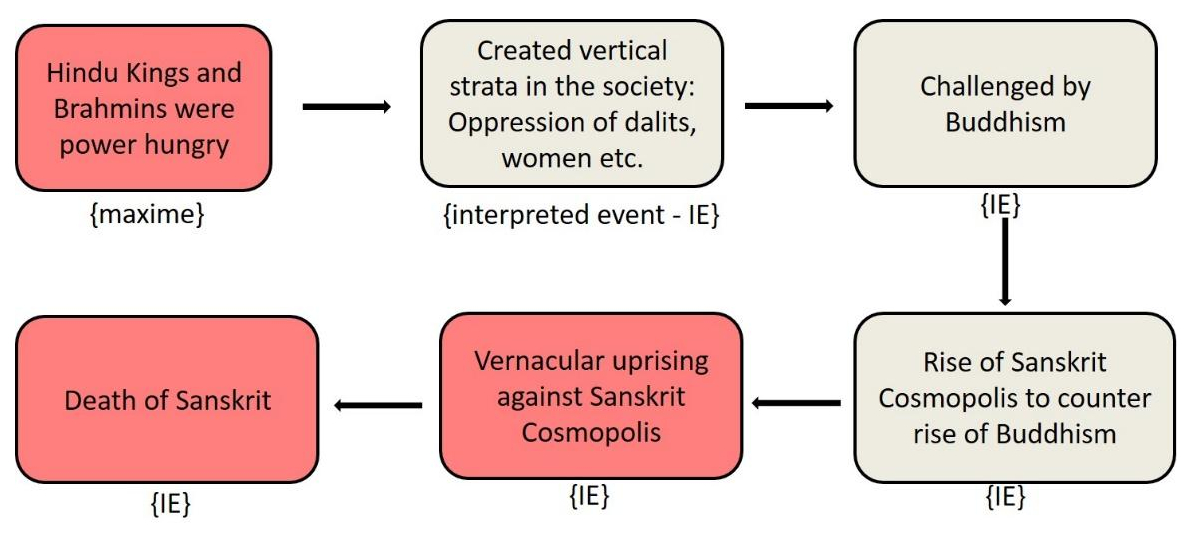
\includegraphics[scale=.22]{images/chap7-1.jpg}
\caption{The schematic shows the narrative and the correlated event hypothesized by Pollock.\index{Pollock, Sheldon} The imposed narrative is that the Hindu kings and the brahmins have always been power hungry, they colluded to maintain the power structure. The red colored boxes (the essential narrative and the interpreted event {IE}) are challenged in this paper.}\label{chap7-fig1}
\end{figure}

Figure 1 clearly shows that chronology plays an important role in this narrative-event correlation. Furthermore, the Western study of humanities and social sciences promises ‘science’. Just as in physical sciences there is a cause-effect correlation, likewise, a cause is assigned (or assumed), and the event is then explained on the basis of that cause. This is akin to the ‘apple falling due to gravity’ explanation. Gravity (which is the cause) must exist for the apple to fall (the event). Thus a science-like study is offered. Moreover, the chronology\index{Chronology} is obvious – gravity must exist/come before the fall of the apple (event).

\subsection*{Approach for This Paper:}

The standard chronology study is performed by checking the veracity of dates for the events. For example, were the \textit{Rāmāyaṇa}\index{Ramayana@\textit{Rāmāyaṇa}} and the \textit{Mahābhārata}\index{Mahabharata@\textit{Mahābhārata}} written ‘after’ Buddhism\index{Buddhism} to counter it? A variation of this study can be – Were these dates researched by Pollock himself, or did he borrow these dates from elsewhere? Is there universal acceptance of these dates? In other words, how established are these dates? These and similar questions offer a rich avenue of research and it has been carried out. For instance, Sastry and Kalyanasundaram’s joint paper (in this volume) investigates this line of questions.

The current paper however takes a different approach. A critical part of assigning the chronology are the actual events themselves. An alternative approach to studying the chronology therefore is to assess this entire sequence of events, a study to verify the accuracy of these events. For instance: Was there even a Sanskrit Cosmopolis?\index{Sanskrit Cosmopolis} Did vernaculars really rise against Sanskrit? etc. – these are some of the questions that can be asked. Taking this approach, this paper looks at the main narrative (power-hunger of kings and brahmins) and the two downstream events imposed by Pollock viz. “vernacular uprising” and “the death of Sanskrit”. The ideas challenged in this paper are marked in red color in Figure 1.


\subsection*{Pollockian Narrative Extends Beyond Time and Space:}

The basic narrative of Pollock\index{Pollock, Sheldon} goes beyond time that he has specified in his Sanskrit Cosmopolis\index{Sanskrit Cosmopolis} (as ~300 C.E. to 1300 C.E.). This is so because the narrative assigned is the inherent flaw, almost as if by design, in the thinking of the Hindu kings and the brahmins – hunger for power. Since it is inherent, it is not limited by time or indeed by space. Accepting this idea for the time being that the Hindu kings and brahmins’ minds have been afflicted with greed, would \underline{not} change with time and space. As such, their acts (events) should reflect this behavior at any point in time and space. Indeed, Pollock is pointing out to this afflicted mind of King Harṣa in Kashmir in the 14th century which he then claims was the cause of downfall and death of Sanskrit in the Kashmir. “It was a century that began with the atrocities of King Harsha” (Pollock 2001: 399). Note that the case of Kashmir is after – beyond - the Sanskrit Cosmopolis. In other words, Pollock himself inherently asserts that his narrative holds across and beyond his Sanskrit Cosmopolis.

The approach of the current paper is that lives of brahmins and kings from a specific time period and space are presented. The time period selected is after the ‘demise of the Sanskrit Cosmopolis’ and extends up to close to the 20th century. The space selected is the center of learning with a long history of the presence of brahmins – viz. Kashi. Hence the title ‘Beyond the Sanskrit Cosmopolis’.

It is shown that Pollock’s narratives and his interpreted events do not match the historically documented accounts of the lives of the brahmins and the Hindu kings, at least in and around Kashi and in the time period studied. Of course, it is recognized that this is a small sample and more research along similar lines is required to form a more comprehensive response to Pollock’s hypothesis.

\newpage

\section*{Prior Challenges to Pollock}

The current paper is obviously not the first work to challenge Pollock’s hypothesis on the death of Sanskrit. Here the critiques by Indologist Hanneder and Sastry are briefly presented.

\subsection*{Hanneder:}

Hanneder has critiqued Pollock’s paper “Death of Sanskrit” from several different positions – definition of death, wide usage of Sanskrit in the ‘Cosmopolis’,\index{Sanskrit Cosmopolis} Pollock’s judgement on quality of Sanskrit works and their quantity, interpretation employed by Pollock and on Pollock’s description of Kashmir and Vijayanagar on the basis of which he, i.e. Pollock, comes to a certain conclusion about Sanskrit in India. Some of these are worth restating.

Hanneder points out how Pollock has arbitrarily prescribed a ground for ‘living Sanskrit’ (opposite of death) viz. “if and only if there is a large quantity of Sanskrit of high quality with a significant influence over a wide space” (Hanneder 2002: 299). Pollock\index{Pollock, Sheldon} then checks against these criteria - based on epigraphs, some texts from Sanskrit poets of the past, and his definitions of quality and influence - and pronounces Sanskrit as dead because one or more of his choice of criteria has not been satisfied. Hence the entire hypothesis is based on self-defined definitions and specific interpretations.

\begin{enumerate}
\item Death 

 While Hanneder\index{Hanneder, J.} agrees that Sanskrit literary production has fallen, he also admits that these might have happened numerous times in the long history of India, the important point being that Sanskrit ‘re-invents’ (Hanneder 2002:~294) itself. He critiques Pollock’s attempts to artificially magnify these discontinuities in Sanskrit literary productions and label them as ‘death’. He also calls out Pollock’s dilemma - ‘Sanskrit is dead in some crucial way’ (Pollock 2001:~393) - pointing out that Pollock himself sees a problem with the word ‘death’. In addition, Hanneder questions this term when, he points out, several writings sprang within a century (within the context of Kashmir) after Sanskrit ‘reinvented’ itself.

 \item Quality 
 
 Hanneder has criticized Pollock on his (Pollock’s) idea of quality of Sanskrit texts in a number of ways (Hanneder 2002: 295). A brace of important ones merit repetition. Firstly, Hanneder quotes Johannes Nobels who openly states that the traditional view of \textit{kāvya}\index{kavya@\textit{kāvya}} must be considered, for these are written with a certain force of creativity\footnote{ Originally written in German. Extract from the translation is presented in italics in the main text.}. This quote from Nobels, which Hanneder (2002: 301) has presented in full, is reproduced here in translated words.
\end{enumerate}

\begin{myquote}
The writer [the author that Nobel is critiquing]…was also not able to manage to illustrate the history of Indian poetry in its development properly….he did not use the correct method, … he does not see the importance and most of all because he does not show the familiarity with Sanskrit, which is required for a good understanding from the inside (i.e. the traditional view). Nobel later states, “We have to basically immerse ourselves into the middle of the Indian world of ideas…to see how each poet draws up the lines…with his genius…and elicits every time, a different shade of color”.
\end{myquote}

Moreover, Hanneder rightly points out that the judgement of quality cannot be an objective criterion to assess. For instance, Upadhyaya,\index{Upadhyaya, Baldev} a traditional scholar of great repute, whose intellectual achievements and works are drawn upon from and presented in the latter half, is in wholesome praise of the \textit{kāvya} texts - and indeed other prose and poetry texts – which Pollock\index{Pollock, Sheldon} brushes aside as being ‘unimaginative’. Thirdly, Hanneder points out that even if the quality was deemed to be ‘lower’, it could have been done purposefully to enhance the activity of Sanskrit at the grass-roots at the time of turmoil (Hanneder 2002: 298).

Hanneder seems to agree with the term ‘Cosmopolis’,\index{Sanskrit Cosmopolis} though he does not agree with Pollock’s assertion of restricted space for Sanskrit in the Cosmopolis. Thus, Hanneder seems to be in agreement with Pollock’s idea of ‘intention to colonize’. Hanneder\index{Hanneder, J.} has also not commented upon Pollock’s assertion that kings and brahmins colluded in such an act of colonization. Thus it is not clear what Hanneder’s position is about the nature of brahmin-king relationship.


\newpage

\subsection*{Sastry:}

\vspace{-.3cm}

Recently, Manogna Sastry has critiqued “Death of Sanskrit” paper by Pollock. Sastry provides several instances in Pollock’s article where his selective citations and interpretations are exposed, and consequently, she rightly questions the motives of Pollock. For instance, in the case of Kashmir, as she extends the efficient critique of Pollock by Hanneder\index{Hanneder, J.} on this case, Pollock is reluctant to discuss the role of Islam\index{Islam} in reducing the Sanskrit related activities in the valley, and this seems to be a general trend in Pollock’s analysis (for example, see Malhotra\index{Malhotra, Rajiv} 2016). Thus, while Pollock is quick to point out Hindu King Harṣa’s destruction of temples, he is conspicuously silent on Sikandar\index{Sikandar Shah Mir} Shah Mir, who went on a rampage, demolishing idols and temples in every village of the valley. Sastry points out that the predecessors of the same King Harṣa, of the Lohara dynasty, continuously provided courtly patronage to Sanskrit and Sanskrit scholars. See Malhotra for further details on the deviant behavior of King Harṣa whose ancestors were more traditional kings, so to speak. Sastry has pointed out multiple instances in Pollock’s paper like the one noted above. In her concluding remark, Sastry makes an important point worth repeating: Pollock’s\index{Pollock, Sheldon} befuddlement in explaining several unanswered questions, not the least his own multiple cases in his article on the death of Sanskrit – “no straightforward manner to configure these four moments in Sanskrit” – is because there is “no naturally connecting thread” that binds these ‘factoids’ together. The corollary of these puzzlements is that Pollock has been forced to be selective in his citations.

Was the expansion of Sanskrit, for example in South East Asia, truly an act of colonization by the Indian rulers, as Pollock asserts - whoever these rulers might have been given that there was no power-center or a center-periphery relation? Were, in the grand narrative, the brahmins and kings power hungry, with a mind-set that would govern their actions? Was there any divide and uprising against Sanskrit in the regional space? Finally, could there be a different interpretation of the observed events, a view different from what Pollock presents, – e.g. in the case of the ubiquitous \textit{praśasti-}s\index{prasasti@\textit{praśasti}} being a brahmin-king nexus as an exercise of power? And yet, all these questions are but a subset of an encompassing larger question: Did Sanskrit ever die? Certainly the traditional scholarship is of the opinion that Sanskrit has always \hbox{been}\break

\eject



 practiced. For one, Ingalls\index{Ingalls, Daniel} is also of the view that Sanskrit activity was very much present.

\begin{myquote}
“The traditions of Sanskrit scholarship, however, was not broken. The brahmins living in the capital or on their tax-free grants of land saw that their sons were taught Sanskrit grammar and the traditional Sanskrit sciences, in many cases teaching their sons themselves.” 

~\hfill (Hanneder 2002: 304)
\end{myquote}

This article aims to submit some historical events from the time period spanning 17th to the 20th century which, as we will see, further supports the view that Sanskrit was indeed very active at the grass-roots of the society. Therefore, in some sense, the article attempts to recreate an image of medieval and pre-modern India based on the documented accounts of Indian scholars and intellectuals, i.e. the pandits. Baldev Upadhyaya’s\index{Upadhyaya, Baldev} book \textit{Kāśī ke Paṇḍiton kī Pāṇḍitya Paramparā} has already been referred to. The entire book and indeed the very existence of such a book, its title \textit{Pāṇḍitya Paramparā}, forms a formidable response to Pollock’s\index{Pollock, Sheldon} assertions. However, for the purposes of a scholarly response, some ‘hard’ facts must be presented. As such, out of more than100 Kashi pandits’ lives accounted for in the book, a few have been chosen for this article.

\vspace{-.3cm}

\subsection*{Pollock’s Befuddlement:}

There are certain events that befuddles Pollock. His befuddlements are: 1) no centre-periphery relationship, a fluid center, 2) no march of military, and 3) no religious crusade, and 4) the large number of \textit{praśasti}-s\index{prasasti@\textit{praśasti}} written. Sanskrit Cosmopolis\index{Sanskrit Cosmopolis} and aesthetic power of Sanskrit offers answers to these befuddling questions. For instance, it explains how Sanskrit (might have) travelled. However, these hypotheses must be examined. Initial critiques by Hanneder,\index{Hanneder, J.} Sastry and Malhotra\index{Malhotra, Rajiv} already cast doubts on Pollock’s hypothesis. In the following, it will be further shown that based on Upadhyaya’s documented evidence of the lives of brahmins and kings, Pollock’s hypothesis seems even more tenuous.

\vspace{-.3cm}

\section*{Further Challenges: \textit{Uttara-pakṣa}}\index{uttarapaksa@\textit{uttara-pakṣa}}

As stated, a lot is drawn here from Baldev Upadhyaya’s book \textit{Pāṇḍitya Paramparā}. It simply documents daily accounts of pandits – from C.E. 1200-1950, and Kashi kings. This is from around the time Sanskrit Cosmopolis has been defeated, according to Pollock, and Sanskrit and the regional vernaculars have fought against each other, with the vernaculars emerging victorious signaling the end of Sanskrit Cosmopolis.\index{Sanskrit Cosmopolis} Sanskrit dies soon after – at different times in different places, 13th century in Kashmir, and mid-19th century in Bengal – ‘on the eve of colonization’ (Pollock\index{Pollock, Sheldon} 2001: 395). The article explores what the documented accounts of pandits and kings tell us.

\vspace{-.3cm}

\subsection*{Who is Baldev Upadhyaya\index{Upadhyaya, Baldev} and \hfill\break What is His Source of Information?}

Before we look at the documented accounts, a note on Baldev Upadhyaya merits attention. He was a Kashi Paṇḍit himself, born in 1899 and passed away in 1999. He edited 9 Sanskrit texts, was the chief editor of 11 more Sanskrit texts. He has written over 30 books in Hindi which are tabulated in the Annexure. He won a number of awards, including a Padma Bhushan award in 1984, a top honor bestowed by the Government of India. Given his literary and intellectual achievements it would be remiss to not state that he was one of the topmost traditional scholars who had profound knowledge about the Indian \textit{samāj} and \textit{sabhyatā}, i.e. Indian civilization and society.

What was the source of his information of the daily accounts of these pandits? A number of his accounts are based on first-hand information because he lived with and studied with or was taught by some of these pandits. In other cases, he has referred to some texts that give the description of these pandits, for instance, Mark Twain’s\index{Twain, Mark} description of Bhāskarānanda\index{Bhaskarananda Sarasvati@Bhāskarānanda Sarasvatī} Sarasvatī (in \textit{More Tramps Abroad}) or Pandit Gopinath\index{Kaviraj, Pandit Gopinath} Kaviraj’s \textit{Kāśī kī Sārasvat Sādhanā}. He also provides a list of texts etc. he has referred to. In still other cases, he has learnt about these pandits from the older scholars who, in their own young days, personally knew some of these pandits.

In the following, are given multiple seemingly simple accounts, which are nevertheless of grave importance, as they tell us of the life of the pandits at the grass-roots – level which is indeed the true indication of a society\endnote{Here are some additional notes about Baldev Upadhyaya\index{Upadhyaya, Baldev} worth mentioning. O’Hanlon\index{O’Hanlon, Rosalind} (2010) has referred to Upadhyaya’s work and so has Aklujkar\index{Aklujkar, Ashok} in his articles which appear in \textit{The Paṇḍit}. Aklujkar considers Upadhyaya’s work as the best source to know about the Kashi Paṇḍits. He also acknowledges Sinha’s work on Bengal Paṇḍits as the best work to refer to for Paṇḍits of Bengal. As a matter for research, it would be meaningful to compare and contrast the life-style of the Paṇḍits from two different parts of India, contemporaneous or not.}. In the sequence of this documentation, the first is the salient features of pandits, followed by descriptions of some Kashi pandits, and the pandits from Bengal. This is followed by a short description of the kings of Kashi and their role. \textit{Praśasti}\index{prasasti@\textit{praśasti}} writing seems to be an integral part of Indian literature. Some examples of \textit{praśasti}-s are presented from and for different spheres of the society.


\subsection*{Salient Features of Pandits:}

Upadhyaya writes a few pages on the general characteristics of the pandits, of at least Kashi, and it would be surprising if these characteristics of Kashi pandits did not match those from other parts of India. These pandits were devoted to attaining knowledge, in what can be called \textit{gyān kī sādhanā}, while leading disciplined lives of austerity, sometimes extreme. Upadhyaya\index{Upadhyaya, Baldev} has great respect for these brahmin Kashi pandits because of their humility and modesty; and this, in spite of attaining a most profound knowledge as well as receiving kingly or emperor patronage. Upadhyaya is not alone in his admiration. Franz Kielhorn,\index{Kielhorn, Franz} pleading (to the West?) for saving Sanskrit and the intellectuals (pandits) who carry the knowledge, was much impressed by their humility and modesty.

\begin{myquote}
“It is sad to see the number of great Śāstrīs, distinguished no less for their humility and modesty than for their learning and intelligence, diminish year after year, and to feel that with them there is dying away more and more of that traditional learning which we can so ill dispense with…” 

~\hfill Franz Kielhorn as cited in Aklujkar\index{Aklujkar, Ashok} (2001: 41)
\end{myquote}

The pursuit of knowledge was their main occupation and they would arrive from all over India travelling great distances in order to come to Kashi.

Their daily practice included teaching students for free, sponsored by the kings and the rich businessmen alike. Some renowned pandits would have a long queue of students waiting their turn to learn from their guru till late night. Given such prevalence of learning in the society it is obvious that not all pandits would find favor with the king and only the renowned or the most talented of the lot made it to the king’s court. Also of note is that the rich in the society, other than the king, also provided food and shelter to the students and pandits. Hence Pollock’s\index{Pollock, Sheldon} claims of an exclusive king-brahmin nexus is questionable.

\newpage

\subsection*{A Challenge to the Charge of \hfill\break “Power-hungry Brahmins” and “Vernacular Uprising”}

Life-accounts of four \textit{saṁnyāsin}-s/pandits are provided – Bhāskarā-\break nanda Sarasvatī, Kavīndrācārya\index{Kavindracarya Sarasvati@Kavīndrācārya Sarasvatī} Sarasvatī, Datiyā Svāmī\index{Datiya Svami@Datiyā Svāmī} and Kāṣṭhajivhā Svāmī, which challenge Pollock’s\index{Pollock, Sheldon} assertions.

\begin{enumerate}
\item  “The Army Chief and the Svāmī” – \textbf{Bhāskarānanda Sarasvatī}\endnote{ Upadhyaya (1982: 834--850)}

 \underline{Birth:} Bhāskarānanda Sarasvatī\index{Bhaskarananda Sarasvati@Bhāskarānanda Sarasvatī} was born in 1832 near Kanpur. He was a Kānyakubja brahmin.

 \underline{Studies:} From the age of 8 to 20 years he studied Veda--s, several \textit{śāstra}-s, \textit{darśana-}s,\index{darsana@\textit{darśana}} Pāṇinian\index{Panini@Pāṇini} grammar (Vyākaraṇa), etc. Left home several times after the death of his first baby. Later in his life, during his travels, he was also initiated into the study of Advaita\index{Advaita} Vedānta and Prasthānatraya.

 \textit{\underline{Saṁnyāsa}}:\index{samnyasa@\textit{saṁnyāsa}} After living in Ujjain for several years he came to a small town called Asni in North India, where he was initiated as a \textit{saṁnyāsin} at the young age of 27.

 \underline{Travels:} Following his initiation, he went for an all-India pilgrimage. He continued his renunciate ways and gave up all his belongings including his meagre clothing that he had. He slept under trees, lived along the banks of the river and lived a life of extreme austerity, practicing his meditation and refining his \textit{citta}. He continued his travels and eventually came to Haridwar where he continued his austere lifestyle but at the same time found a \textit{guru}.~After finishing his studies he went to Kashi where he chose a garden to live and perform his austerities. The king of Amethi, who was his student, offered the king’s garden for him to live in instead – Anandbagh. Svāmī accepted and lived in that garden for the rest of his life.

 \underline{Service to the masses:} His compassion for the common masses is seen in this single example where he treated a homoeopathic doctor’s wife (suffering from cholera) and son, following which the doctor became a devoted disciple of Svāmīji.

 \underline{Life accomplishment:} His sense of austerity, \textit{aparigraha}\index{aparigraha@\textit{aparigraha}} (essentially non-attachment), was of the highest order and these austere practices, people believed, gave him special powers. His fame grew far and wide, and he was visited and/or contacted by heads of States/kings, high powered administrative officers, from India and beyond. Yet, he continued his austerities. He was visited by Mark Twain,\index{Twain, Mark} and the German emperor (Wilhelm I) and his grandson sent a note to him (after he had declined the Emperor’s offer to come to Germany) along with his photograph\endnote{ The note reads: “Dear Sir, I have a pleasure in sending you the photos of the Emperor Wilhelm I, the founder of the German Empire and of his grandson, our present Emperor. I wish you health and long life. Your most obedient servant, Gruf Konigs Mark (signed).”}. He treated the rich and the poor, emperors and kings included, the same.

 Upadhyaya\index{Upadhyaya, Baldev} cites several interesting examples including that of the Commander-in-Chief of the British army, namely William Lockhart\index{Lockhart, William}. This army chief, after defeating the Afridis of Afghanistan, came to see the Svāmī accompanied with his wife and a select few junior commanding officers. As they sat down with the Svāmī, Lockhart boasted of his recent exploits. The Svāmī smiled and asked him to lift a pencil which, much to the surprise of the General and others present, the General could not however hard he tried. He bowed to the Svāmī who then proceeded to explain the General the qualities of humility and modesty.

 \underline{\textit{Praśasti}-s:}\index{prasasti@\textit{prasasti}} It is clear that Svāmīji had become very popular and several known personalities visited him for his \textit{darśana}.\index{darsana@\textit{darśana}} After he passed away (he took \textit{samādhi} in 1899) several of his followers came together and wrote several for the Svāmī in Sanskrit and Hindi. The \textit{praśasti}-s seems to be compiled in a single volume.

 \underline{Writings:} Despite his busy schedule with followers wanting his time, and his daily spiritual practices, he did devote some time to writing a few texts. He wrote a commentary on Vedānta called \textit{Svā rājya Siddhi}, commentary on 10 Upaniṣad-s called \textit{‘Prakāśā’},\index{Prakasa@\textit{Prakāśā}} and a brief exposition on the \textit{Nalodaya Kāvya}\index{kavya@\textit{kāvya}}\index{Nalodaya Kavya@\textit{Nalodaya Kāvya}} which appeared in a publication called \textit{Subodhinī}. He also wrote a Sanskrit text \textit{Anubhūti Vivaraṇādarśa}.\index{Anubhuti vivaranadarsa@\textit{Anubhūti Vivaraṇādarśa}}

 \underline{Gleanings:} Several points emerge from Bhāskarānanda Saras\-vatī’s\index{Bhaskarananda Sarasvati@Bhāskarānanda Sarasvatī} life that contradict Pollock’s\index{Pollock, Sheldon} assertions of ‘greedy power hungry brahmins’ and ‘vernacular uprising’ – 1) free movement across India, severe austerity with extreme renunciation, including clothes, 2) simultaneously reasserts Upadhyaya’s points - dedication towards knowledge and \textit{tapasyā} and devotion towards guru, and 3) \textit{praśasti} written for a fellow Pandit as opposed to Pollock’s claim that \textit{praśasti}\index{prasasti@\textit{praśasti}} was written for kings to give them divine status and consequently political power.


 \item 
 “The 600 km Foot-march” – \textbf{Kavīndrācārya Sarasvatī}\index{Kavindracarya Sarasvati@Kavīndrācārya Sarasvatī}\endnote{ Upadhyaya (1982: 77--85)}

 \underline{Birth:} Kavīndrācārya was contemporary with the Mughal emperor Shah Jahan\index{Shah Jahan} and even saw the rise of Aurangzeb\index{Aurangzeb} to power. Thus we can place him in the 17th century. He originally came from the Godāvari region.

 \underline{Studies:} He studied the Veda-s, Vedāṅga-s and other \textit{śāstra}-s. After his studies he too became a \textit{saṁnyāsin} (renunciate).

 \underline{Life:} Kavīndrācārya was good friends with the French traveller and writer, Bernier\index{Bernier}, who describes Kavīndrācārya’s life in some detail. For instance, Upadhyaya\index{Upadhyaya, Baldev} cites Bernier about Kavindracharya’s simple outfit – a white loin cloth (\textit{dhoti}) and a red shawl (\textit{chādar}) on his shoulders being the prominent component. Importantly, he adorned the same outfit whether he was in front of the emperor or on the streets of Agra. Kavīndrācārya used to receive Rs.~2000 as monthly pension from Shah Jahan for his intellectual capacity which, clearly, the emperor was quite taken by. The Svāmī, in turn, would donate all of this money to other brahmins along the banks of the river.

 It is instructive to note here that Pollock,\index{Pollock, Sheldon} who has discussed Kavīndrācārya’s works in “Death of Sanskrit” (Pollock 2001) (and dismissed them as being unoriginal), points to the collection of texts in Kavīndrācārya’s library and attributes it to the pension from Shah Jahan - ‘no doubt thanks to a pension from the Mughal emperor’ (Pollock 2001: 408). This is a good example of how erroneous claims can be made by Indologists in general and by Pollock in particular.

 \underline{Service to the masses:} His compassion for common people is demonstrated by the following incident – a major incident, which even the Western Indologists acknowledge it (see O’Hanlon\index{O’Hanlon, Rosalind} (2010), for example). The incident involves the Hindu tradition of going on a pilgrimage by the common people and ascetics alike, from all parts of India, across all of India. Shah Jahan, the emperor in Agra, imposes a selective tax on Hindus for their pilgrimage. Upadhyaya describes the situation as follows: the pilgrimage, the \textit{yātrā}, was itself an arduous task – a challenge – and to be imposed with a tax on top, created great difficulty for Hindus everywhere. Kashi being the center of learning, came under the attention of people, who looked up to the Kashi pandits to find a solution. Kavīndrācārya, being the most renowned in Kashi at the time, was approached to speak to the Mughal emperor. He readily agreed and along with a few pandit friends to accompany him, started on foot. The distance between Kashi and Agra is ~600 km – a pilgrimage in itself.

 Question to ponder: Why would a Pollockian\index{Pollock, Sheldon} elitist travel 600km on foot, braving hardships? Note that Kavīndrācārya\index{Kavindracarya Sarasvati@Kavīndrācārya Sarasvatī} was yet to meet with the emperor and the patronage of Rs. 2000 per month had not commenced at that time.

 His journey is likened to that of the Sikh guru, Guru Teg Bahadur\index{Guru Teg Bahadur} (executed by Aurangzeb\index{Aurangzeb}), both with a noble cause but one on a horse, with soldiers to accompany and the other with some \textit{svāmī--s} as travelling partners. Once in Agra, at the emperor’s court, he made a forceful case for the abolition of taxes. Upadhyaya\index{Upadhyaya, Baldev} reproduces the note from historian H. P. Shastri\index{Shastri, H. P.} on this incident.

\begin{myquote}
“He journeyed to Agra with a large following and proceeded to Diwânâm and there he pleaded the cause of the Hindu pilgrims, with so much force of eloquence that all the noblemen of the court from Irâk, Irân, Badakshan, Balkh …., were struck with wonder. Shah Jehan and Dara Shikoh\index{Dara Shikoh} relented and abolished the tax [i.e. the pilgrim tax]. That was a day of great rejoicing throughout Hindu India. It was on this occasion that the title of \textit{Sarvavidyânidhâna} was conferred upon him.” 

~\hfill Shastri (1912: 11) (\textit{spellings as in the original})
\end{myquote}

 \underline{\textit{Praśasti}-s:}\index{prasasti@\textit{praśasti}} Even when only Kashi and Prayag pilgrims were absolved of the taxes, there was a group of scholars, 69 of them, who wrote \textit{praśasti} text in honor of him, for Shah Jahan\index{Shah Jahan} and also Dara Shikoh. Therefore, the \textit{praśasti}-s include the respect for Kavīndrācārya as well as for Shah Jahan and Dara Shikoh.

 \underline{Writings:} Upadhyaya contends that Kavīndrācārya could not spend much time writing because most of his time was spent helping the people. However, Kavīndrācārya generated literature, both in Sanskrit and Hindi. There is only one work published, although it is said he wrote a number of works, all unpublished. One of this is the \textit{kāvya}\index{kavya@\textit{kāvya}} text \textit{Kavīndra-kalpadruma} which remains unpublished. The other unpublished Sanskrit texts include \textit{Yoga-bhāskara},\index{Yogabhaskara@\textit{Yoga-bhāskara}} \textit{Śatapathabrāhmaṇa Bhāṣya}\index{Satapatha Brahmana@\textit{Śatapatha Brāhmaṇa}} and \textit{Haṁsadūta Kāvya}\index{Hamsaduta kavya@\textit{Haṁsadūta Kāvya}} (the last one is contested as to whether it was Kavīndrācārya who wrote it). His Hindi texts include \textit{Vaśiṣṭha--sāra}\index{Vasisthasara@\textit{Vaśiṣṭha--sāra}} and \textit{Samaya--sāra}.\index{Samayasara@\textit{Samaya--sāra}}

 Gleanings: If Pollock’s\index{Pollock, Sheldon} writing about Kavīndrācārya’s\index{Kavindracarya Sarasvati@Kavīndrācārya Sarasvatī} pension usage is incorrect, then, how accurate is Pollock’s statement – “…a wide variety of \textit{competing} religious orders, Saiva, Buddhist, Vaiṣṇava, and others”? (Pollock 1996:~198)(\textit{italics ours}). The question raised is for the underlined word ‘competing’. The bigger question to ask is, can the writings of such Indologists be trusted? Additionally, it shows the importance of meticulously performing comparative study of texts written by traditional scholars and Indologists. Furthermore, the act of Pilgrimage Tax imposed on Hindus has an important lesson for this article – the Hindus from across the country travelled from one region of the country to another. This is a significant point worth noting \textit{vis-à-vis} the Pollockian presumed conflict between different regions of India and the Sanskrit Cosmopolis.\index{Sanskrit Cosmopolis} The pilgrimage across India directly contradicts Pollock’s claim of ‘vernacular uprising’ i.e., fight between one part of the country with another or Sanskrit trying to dominate. As far as \textit{praśasti}\index{prasasti@\textit{praśasti}} is concerned, once again we find \textit{praśasti} written for a pandit and non-Hindu king and his son – once again contradicting Pollockian assertion that \textit{praśasti} was used as an instrument of political power. Finally, Kavīndrācārya came from Godāvari region from Southern India and lived in Kashi, and travelled 600km – this again contradicts ‘vernacular uprising’ narrative of Pollock.

 \item  “The Energetic Pilgrim” – \textbf{Datiyā Svāmī}\index{Datiya Svami@Datiyā Svāmī}\endnote{ Upadhyaya (1982: 873--881)}

 \underline{Birth:} The childhood name of Datiyā Svāmī was Mahāvir Prasad, born not far from Kashi, in 1898. He was a Saryuparin brahmin.

 \underline{Studies:} In 1913, he left his home at the young age of 15 and came to Kashi to study Sanskrit. He studied Vyākaraṇa under a \textit{guru,} and soon came in contact with another Svāmī living in a small hut nearby. The contact with the Svāmī flowered a deep sense of taking up \textit{saṁnyāsa},\index{samnyasa@\textit{saṁnyāsa}} which he eventually did, and was initiated into renunciation by the same Svāmī. On the other hand, he continued his study of {Veda--s, Vedānta} and several \textit{śāstra-s}.

\newpage

 \underline{Life:} His father died at a very young age. His mother would carry him on her shoulders to the nearby goddess Kālī temple which nucleated a strong desire in the boy towards a \textit{sādhana} for Śakti. As he grew older, he would visit a Hanumān temple every day and, evidently inspired by the deity, even took up wrestling. He went to a school for his initial education. He studied, among other subjects, Urdu and quite liked it. Later on his life, during his pilgrim travels no doubt, he became quite a polyglot with fluency in Bengali, Marathi, Gujarati, Punjabi and other local languages. That was to come much later though. He was also a fan of music and enjoyed listening to different genres of music including Sufi\index{Sufi mysticism} mysticism. He even wrote ghazals in Urdu. Notably, one of his disciples wrote a ghazal in Urdu and was blessed by him.

 \underline{Travel:} In 1926, after a study spanning 13 years, he set out on a pilgrimage to deepen his spiritual quest. He visited Kangra, Bengal, Bombay, Nepal, etc. and finally reached Punjab. He met a Gujarati \textit{saṁnyāsa}, Ananthanandanath, who initiated him in Tantric practices. Under the advice of his guru, the Gujarati \textit{saṁnyāsin}, he set himself along the banks of river Narmada and did \textit{tapasyā} for one whole year. He then continued his travels to Amritsar, Tarantaran, Dhaulpur, etc. and eventually reached Datiya\index{Datiya Svami@Datiyā Svāmī} in Madhya Pradesh in 1929. He stayed there for the next 50 years till his death. He continued his practice of Tantra there. Like Bhāskarānanda Sarasvatī,\index{Bhaskarananda Sarasvati@Bhāskarānanda Sarasvatī} he attained \textit{samādhi} in 1979.

 \underline{Service to masses:} In Datiyā, he performed several service for the common masses. He established the Bhagavatī Pītāmbarā in 1935, which became popular as an \textit{āśrama} in all of India. Earlier he had established a temple for Paraśurāma, and was considered a great scholar of \textit{Śāktamata}. The remarkable thing being that Paraśurāma is traditionally mostly revered in Maharashtra and Kerala, but to establish such a temple successfully in Madhya Pradesh speaks of the respect people had for this Svāmī. Additionally, while a temple for Reṇukā, Paraśurām’s mother, exists in Kashi, no temple for Paraśurāma exists even in Kashi. Other temples included those of Mahākālabhairava, Dhūmavatī and Tārā. Special mention must be made of the Ṣaḍāmnāya Śiva’s temple – a rarity, given that it is hardly found anywhere else in India. He proceeded to consecrate six idols of Shiva corresponding to the six-named Śiva (Ṣaḍāmnāya) in an ancient temple in Vankhandeshwar in 1980.

 He was adept at Vedic and Tāntric \textit{yajña}-s.\index{yajna@\textit{yajña}} He was not only a great proponent of British-free India but also performed a Rāṣṭra-rakṣā \textit{yajña} (National Safety \textit{Yajña}) when China attacked India in 1961. He also performed a Brahma-yajña where 9 days were allotted for each of the four Veda--s and the \textit{yajña} carried on for 36 days. The first \textit{yajña}, i.e. the National Safety \textit{Yajña}, was performed with Tantric rituals; and the second, the Brahma-yajña, with Vedic rituals. While one may not subscribe to the idea of performing \textit{yajña}-s for beneficial purposes, no one can deny the societal awareness that Datiyā Svāmī\index{Datiya Svami@Datiyā Svāmī} displayed, and the sense of duty towards his country and fellow human-beings. Like Bhāskarānanda Sarasvatī,\index{Bhaskarananda Sarasvati@Bhāskarānanda Sarasvatī} he acquired inexplicable powers through his devoted Tāntric practice, which he used, for example, for treating the terminally sick.

 \underline{Writings:} Like Kavīndrācārya\index{Kavindracarya Sarasvati@Kavīndrācārya Sarasvatī} and Bhāskarānanda, he too wrote a significant number of texts. He wrote instructions for\break offerings for the deities he established in several temples,\break commentaries on several ancient Tantra texts, and those related with new findings. For instance, he wrote descriptions of\break ancient texts while simultaneously writing new texts shows. In\break particular, he advocated similar forms in the Āgama-Nigama\break texts, and he would see elements of Āgama in the Vedic\break \textit{mantra}-s. According to Upadhyaya,\index{Upadhyaya, Baldev} such findings of Datiyā Svāmī are new and independent and which Upadhyaya contends,\break Datiyā Svāmī’s view that there is unity in diversity

 Gleanings: Such multilinguality is found amongst great many pandits, a number of whom wrote in Sanskrit, Hindi and other languages. Note the inter-regional co-operation amongst the \textit{saṁnyāsin}-s. Notice once again the popularity across regions throughout India. This popularity of an \textit{āśrama} would not have happened through state-sponsored advertisement, that too in pre-Independence India, but only through visitations by the common masses. In other words, the visitations by common masses from across different regions would have been the source of such popularity.

\newpage

 \item 
 ‘The Wooden Sleeve’ – \textbf{Kāṣṭhajihvā Svāmī}\index{Kasthajihva Svami@Kāṣṭhajihvā Svāmī}\endnote{ Upadhyaya (1982: 791--806)}

 Kāṣṭhajihvā Svāmī was the \textit{guru} of Kashi King Ishwari Prasad Narayan Singh – a king of exceptional intelligence with a sincere devotion towards the pursuit of knowledge. Kāṣṭhajihvā Svāmī was a very modest person. It is said that once he uttered some words in anger, \textit{apaśabda}, against a senior monk. He was filled with much remorse, and to prevent himself from poor utterances again, especially those directed against his peers and seniors, he put a wooden sleeve on his tongue – hence his name Kāṣṭhajihvā (“wooden tongue”). This act is unusual, extraordinary and likely is unparalleled.

\vspace{0.1cm}

 \underline{Writings:} Upadhyaya\index{Upadhyaya, Baldev} sees Kāṣṭhajihvā Svāmī in two roles: one as a \textit{sādhaka} (spiritual seeker) and the other, a poet. Though his role as a poet is relatively well known, his role as a \textit{sādhaka} is not so well known. His favorite acolyte was none other than the Kashi King Ishwari Prasad Narayan Singh, who himself was a great devotee of his \textit{guru} and a serious scholar. Kāṣṭhajihvā Svāmī wrote both Sanskrit and Hindi texts. His enumeration of Sanskrit texts is counted at 21, although, Upadhyaya states, one British author has only mentioned 4 of these. None of his publications, Sanskrit ones, have been published, and only the handwritten manuscripts remain. His Hindi texts are many, some published and some unpublished. \textit{Rāmāyaṇa Paricaryā}\index{Ramayana@\textit{Rāmāyaṇa}}\index{Ramayanaparicarya@\textit{Rāmāyaṇa Paricaryā}} is one of his most significant works. Although he was a \textit{sādhu}, he was also a poet.

\vspace{0.1cm}

 \textit{Rāmāyaṇa Paricaryā} is more a note than a commentary on the essence of the \textit{Rāmāyaṇa}. Upadhyaya notes the necessity of reading the entire text, but quotes Kāṣṭhajihvā Svāmī on some details such as – why Sundara Kāṇḍa was named so etc. It makes for a difficult reading which prompted King Ishwari Prasad Narayan Singh to write a commentary on the \textit{Paricaryā} to make the \textit{Paricaryā} comprehensible. It was called the \textit{Pariśiṣṭa}.\index{Parisista@\textit{Pariśiṣṭa}} This is a pointer to the high calibre of intellect of Ishwari Prasad Narayan Singh. This commentary too was not simple enough for the common masses. Thereby a third person, cousin of the Maharaja – Śrī Harihar Prasad - wrote a simpler version of the \textit{Pariśiṣṭa}. It was called \textit{Prakāśa}.\index{Prakasa@\textit{Prakāśa}} The three of them together was published in 1896 under the name \textit{Rāmāyaṇa-Paricaryā-Prakāśa-Pariśiṣṭa}. Similarly, Kāṣṭhajihvā Svāmī wrote \textit{Kāśīrāja-Sāgara}, a Sanskrit text, which too, Upadhyaya contends, is quite difficult to comprehend for the modern pandits.

\vspace{0.1cm}

 Gleanings: The short description of Kāṣṭhajihvā Svāmī\index{Kasthajihva Svami@Kāṣṭhajihvā Svāmī} and his student King Ishwari Prasad suggests the humility of the pandit on the one hand, and a strong penchant for knowledge and a desire to help the common masses in the king on the other. Else, this Hindu king would not have attempted a commentary for easier comprehension of the \textit{Paricaryā}.\index{Ramayanaparicarya@\textit{Rāmāyaṇa Paricaryā}} This negates Pollock’s\index{Pollock, Sheldon} hypothesis of power hunger in kings and brahmins.

\vspace{0.1cm}

 The few exemplary descriptions clearly show that these pandits, across space and time, demonstrate a single minded devotion to the pursuit of knowledge – all in Sanskrit – attained through hard work and discipline. These pandits are from different centuries, thereby pointing to a continuity of tradition. Notice that these pandits are within the time-line of the presumed Pollockian ‘Dead Sanskrit’ – Kavīndrācārya\index{Kavindracarya Sarasvati@Kavīndrācārya Sarasvatiī} appearing in the tumultuous time of Aurangzeb\index{Aurangzeb} and the colonizing British are yet to arrive. Regardless of the centuries that have passed between these pandits, and although only four examples are discussed, reading Upadhyaya\index{Upadhyaya, Baldev} shows that the picture that emerges of brahmin pandits is one of intense yearning for knowledge and subsequent dissemination of the same. For instance, Pandit Gopi Nath, his son Gokul Nath and his student Manidev wrote \textit{Mahābhārata Darpaṇa}.\index{Mahabharatadarpana@\textit{Mahābhārata Darpaṇa}} It is approximately 2000 pages and took about 50 years to complete. Such was the pursuit of knowledge of the pandits.

\vspace{0.1cm}

 Furthermore, this is a good indication of the activity of Sanskrit at the grass-roots – the so-called ground-reality. Even when Islamic\index{Islamic rule} rulers, a number of them, had imposed themselves on the Hindus, and the trend continued with the British – for example, Warren Hastings, who attacked Kashi with his forces, but was forced to retreat in the cover of the night – Sanskrit was still being taught, learnt and expressed in texts.
\end{enumerate}


\newpage

\subsection*{Kashi Kings: \hfill\break Challenge to the Narrative of “Power- hungry Kings” \hfill\break and “King-Brahmin Collusion to Impose”}

Table II collects the description of Kashi kings. Although Upadhyaya\index{Upadhyaya, Baldev} describes the full lineage, for the sake of brevity, this lineage is shortened for this article. Column III in the table shows the king’s main accomplishment and the corresponding counter narrative to Pollock is provided in column IV. A quick glance at the table suggests valiant, intelligent Hindu kings who fought against aggressors, restored order in the society (often caused by alien rulers – Muslim or British) and provided patronage to brahmin/non- brahmin scholars alike. These attributes of the Hindu kings is almost impossible to reconcile with the Pollockian narrative of the Hindu kings.

\vspace{-.3cm}

\subsection*{Cross-regional Culture: \hfill\break Challenge the “Vernacular uprising” and \hfill\break “Death of Sanskrit” Hypothesis of Pollock}\index{Pollock, Sheldon}

\vspace{-.2cm}

Here, the interconnectedness between Bengal-Kashi is briefly explored. Kashi pandits were asked to move to Calcutta and teach in the Sanskrit college of Calcutta. This demonstrates a strong cross-regional culture. While Kashi Sanskrit college was established in 1791, the Sanskrit college in Calcutta was established in 1824. There are two obvious facts but worth stating – the opening of Sanskrit colleges. Some may argue that this was done by the British to help revive Sanskrit. However, running the Sanskrit college actually depended upon Sanskrit pandits. It was these pandits, home grown through a lineage called \textit{Pāṇḍitya Paramparā}, who were hired to teach Sanskrit in these colleges. What allowed the existence of such \textit{paramparā}, yielding such pandits to run the Sanskrit colleges if Sanskrit was dead by 1300 – “Sanskrit lost these contests \textit{(with vernaculars)} and lost them everywhere” (Pollock 1996: 198) – as Pollock describes it? What actually emerges is that Sanskrit pandits were still learning their \textit{śāstra}-s within the \textit{guru-śiṣya paramparā} and appointments in Sanskrit colleges were simply a matter of a regular source of income, which in the earlier times were provided by the kings and the rich business men. An alternative way to ask the question is - would these Sanskrit colleges, albeit helped in their inception by the British, have any meaningful existence if there were not Indian Sanskrit pandits already available to run them? Here is an example from British administrators seeking and utilizing Indian pandits for running the Sanskrit colleges. The following example is a letter of recommendation for a job for Paṇḍit Nāthuram Śāstry\endnote{Another example is that of Paṇḍit Krishnadev Upadhyaya. He taught Vedānta Philosophy to W. H. Mill of the Bishop college.}:

\begin{myquote}
“The secretary beg to propose Nāthu Rāma, a Paṇḍit of considerable abilities for the office as a fit person to succeed to the appointment. The individual in question was in the college of Banaras, where he bore a high character. He lost his appointment there, in consequence of exceeding his leave of absence which it subsequently appeared owing to family distresses and not to any improper neglect (24th July, 1827).”
\end{myquote}

Hanneder\index{Hanneder, J.} has already commented upon the selective interpretation of Pollock\index{Pollock, Sheldon} regarding Bengal. A few more examples will illustrate the error in Pollock’s analysis, not only of a “dead Sanskrit”, but also of a society where knowledge in Sanskrit was still considered important.

\textbf{Yadaveśvara Tarkaratna}: b.~1850 in North Bengal, d.~in 1924. Initially learnt Bangla in his village. He also learnt Sanskrit in Bengal itself from Haragovinda Siddhānta (grammar), Īśvara Vidyālaṅkara (\textit{Kāvya Prakāśa}).\index{Kavyaprakasa@\textit{Kāvya--prakāśa}} His father died when he was only 5, but his father’s students made sure he did not feel orphaned. They arranged for him to go to Kashi for further studies. There he learnt Nyāyaśāstra\index{Nyaya@Nyāya} from Kailāśa Candra. It was his excellence in Nyāyaśāstra that gave him the title of Tarkaratna. He then went to Svāmī Viśuddhānanda Sarasvatī and learnt Vedānta and Yoga\index{Yoga} Darśana.\index{darsana@\textit{darśana}} Griffith called him and taught him Western philosophy. He then went back to Rangpur where he joined as a teacher in a school where he taught Sanskrit. It must be noted here that a school in Bengal in a small village was teaching Sanskrit. This school closed down (for some reason), and he with the help of Śrī Aurobindo’s father, started a Sanskrit school.\index{Sanskrit schools} In this new school he taught \textit{kāvya},\index{kavya@\textit{kāvya}} grammar and \textit{śāstra}. It is thus difficult to accept Sanskrit as a dead language, at least during this period.

He was felicitated both for his Sanskrit works and his service to Bangla. This clearly shows that both Bangla and Sanskrit happily co-existed at the eve of colonization. His creations were, expectedly, both in Sanskrit and Bangla. Sanskrit creations include: \textit{Śoka-taraṅgiṇī} (a \textit{kāvya} piece), \textit{Vāṇī-vijaya}, \textit{Subhadrā-haraṇa} and ten more. Bangla creations include: \textit{Draupadīkāvya}, \textit{Aśoka}\index{Asoka@Aśoka} (a novel) and a few more. His only son was a scholar too who wrote about Jain images (a Hindu writing about Jain deities must be noted) – written in English, and \textit{Sārnāth kā Itihās} in Bangla. It seems language was not an issue at all. These scholars wrote in whichever language they felt at home with and obviously were usually well read.

\textbf{Vidhuśekhara Śāstrī}: He was a Buddhist scholar. He learnt Hindu \textit{śāstra}-s as well as Buddhism\index{Buddhism} texts – all in Kashi. He too was born in Bengal (Maldah) in 1878 and was born in a brahmin family. He first learnt English in a local school, and later, on his father’s insistence, went and learnt Sanskrit as well (\textit{kāvya})\index{kavya@\textit{kāvya}} in Bengal itself. He wrote two small texts on \textit{kāvya}. He then went to Kashi and learnt \textit{śāstra}-s.\break He learnt Nyāya\index{Nyaya@Nyāya} from Kailāśa Candra Śiromaṇi and Vedānta from Subrahmaṇya Śāstrī. Vidhuśekhara was influenced by European scholars and was inspired to learn about Buddhism. He learnt Tibetan, and wrote a grammar book on Tibetan. He and his students translated Buddhist texts in Tibetan into Sanskrit. This one example ought to be enough to see that Sanskrit at grass-roots in Bengal was very much alive. His writings – too many to list here – were in Bangla, Sanskrit and English, noteworthy being books on Tibetan grammar, translation of Gauḍapādācārya’s Advaita\index{Advaita} Vedānta etc. Once again, notice the multilinguality and free movement across different regions of the country. Similar examples may be seen in the life accounts of \textbf{Kshiti Mohan Sen, Vaidyanath Mishra} etc. who studied Sanskrit, and wrote in a host of different languages – Hindi, Bangla, and English.

It is a sign of remarkable harmony within the society that a brahmin Pandit became a Buddhist scholar. This evokes a sense of camaraderie between brahmins and Buddhists, and a permeable interface between brahmins and Buddhists, or between scholars with inclinations towards different texts of authority. Take for example the case of a Jain scholar helping Upadhyaya\index{Upadhyaya, Baldev} with his book \textit{Ārya Sanskṛti ke Mūlādhār} (Upadhyaya 1947). Also of note is the incident presented by Upadhyaya where a group of brahmin scholars came together to help with the Theosophical Society in 1880 (Upadhyaya 1982:~140). Also, Tarkaratna’s son, being a brahmin, wrote freely on Jain images.

\newpage

\textbf{Table 1. Lineage of Kashi kings and their main accomplishments. Counter narrative to Pollock's\index{Pollock, Sheldon} ideas is also provided.}

\begin{longtable}{|p{1.4cm}|p{1.6cm}|p{2.6cm}|p{2.6cm}|}
\hline
Kashi King & King’s learnings & King’s main accomplishments & Counter narrative to Pollock \\
\hline
Rama Sharma – was a brahmin & Learnt Sanskrit and weaponry. & Defeats the rogue elements in the surrounding areas of Kashi. & A brahmin performing \textit{kṣātriyic} activity points to a horizontal/fluid \textit{varṇa}\index{varna@\textit{varṇa}} system. \\
\hline
Mansārām &   & With the help of his younger brothers defeats the then Muslim rule in the Kashi region - the society was riddled with robbery, theft and insecure life. & A valiant and intelligent Hindu King brings social order during the time of unrest in the society. \\
\hline
Balwant Singh &   & Extends the kingdom, moves the capital to Ramnagar, builds a fort, Śiva temple; in association with Rāṇī Ahilyā reconstructs the Kashi Viśvanātha temple. & He brought the temples, especially smaller ones, to a more functional status e.g. ringing bells. Gave patronage to both Hindu and Muslim scholars (Sheikh Ali-Haji who fled from Nadir Shah’s atrocity). \\
\hline
Cet Singh & Sāhitya & He fought Warren Hastings – the population of Kashi, in support of Cet Singh, rose in revolt against Hastings who had to beat a retreat. & Service to the masses who preferred a Hindu king’s rule over Warren Hastings. \\
\hline
Mahip Narayan Singh &   & Donated land for Government Sanskrit school.\index{Sanskrit schools} Largely quelled the turmoil and unrest (possible British influence) during his time. & Service to the masses. \\
\hline
Udit Narayan Singh & Wrote three commentaries on the \textit{Rāmāyaṇa}.\index{Ramayana@\textit{Rāmāyaṇa}} & He started the Rāmlilā tradition which is still followed today. He also ordered pictorial representation of the \textit{Rāmāyaṇa} which is unique. & His younger brother built gardens around the city for general population. These are direct evidences of service to the masses. \\
\hline
Ishwari Prasad Narayan &   & Saved cows from a butcher by buying them overpriced. Wrote a commentary on the difficult-to-understand \textit{Rāmāyaṇa Paricaryā}.\index{Ramayanaparicarya@\textit{Rāmāyaṇa Paricaryā}} & Confiscating cows would have been an act of demonstrating power. Buying the cows, on the other hand, was a demonstration of fairness. \\
\hline
\end{longtable}


\section*{Clash of Narratives}

\subsection*{Pollock’s\index{Pollock, Sheldon} View of Indic Civilization Revisited:}

Pollock’s statement of melancholic Indian history notwithstanding for the time-being, his image of pre-modern India indicates the period between 800-1300 CE of great turmoil when regional forces grew against Sanskrit Cosmopolis\index{Sanskrit Cosmopolis} and defeated Sanskrit everywhere – “…with reference to Sanskrit’s complicated contests with regional languages… Sanskrit lost these contests and lost them everywhere” (Pollock 1996: 198). Following these ‘contests’ Sanskrit Cosmopolis was ‘destroyed’ and subsequently, the death of Sanskrit ensued. However, the few scattered historical accounts presented in this paper already begin to dismantle this hypothesis. We already see a substantial and continuous Sanskrit activity as late as 20th century contradicting Pollock’s assertion of a “dead Sanskrit” – Datiyā\index{Datiya Svami@Datiyā Svāmī} Svāmī, whose works were deemed to be new by Upadhyaya\index{Upadhyaya, Baldev}. Moreover, we also see translations of original Sanskrit texts in Hindi, that is Upadhyaya’s texts, and their subsequent translations not only in Indian vernaculars, Kannada and Telugu etc., but also in ex-Indic languages Burmese and Sinhalese. The relevance of these two neighboring regions translating Upadhyaya’s texts is not lost, as Pollock has cited two holes in the Sanskrit Cosmopolis – Burma and Sri Lanka! Clearly, Pollock is inaccurate with regards to Burma and Sri Lanka within his own Cosmopolis. More remarkable is the thriving Sanskrit activity at the grass-roots with home-schooling of pandits in Sanskrit followed by tutelage with a \textit{guru}. As the State patronage installed by the Kings declined, the brahmins have been forced to abandon their traditional life-styles – that of single-minded pursuit to knowledge and freely disseminating it for the future generations.

One relies on such books as Upadhyaya’s to get a more accurate sense of what the society must have looked like with the brahmin community’s devotion to their pursuit, not of power, but of knowledge, through and sometimes beyond, what may be termed a drastic change in the nature of relationship between the ruler and his subjects - first with the coming of Islam,\index{Islam} and then of the British colonialism. Were there a few brahmins who fell into greed, and did not follow the traditional path? Surely, there would have been some. But ‘some’ does not constitute the ‘whole’. The picture recreated by Indologists should be on the ‘statistically significant’, so to speak, as opposed to the ‘statistically negligible’. My preliminary conclusion is that more the details compiled from such books as Upadhyaya’s, the shakier Pollock’s hypothesis would turn out to be.


\subsection*{Traditional View of Indic Civilization:}

Several questions have baffled Pollock,\index{Pollock, Sheldon} which he concedes to too, and then answers them through “aesthetic power of Sanskrit and Sanskrit Cosmopolis”.\index{Sanskrit Cosmopolis} However, several of his interpretations and conclusions have been critiqued substantially. What could be a unifying theory that explains all the observed events? Could a traditional view of the Indic society offer some help to these seemingly unanswerable questions?

Following is the traditional view-point of the Indic society. Upadhyaya\index{Upadhyaya, Baldev} states that the Indic society has been a product of an interplay between Jain, Buddhist and Vedic philosophical thoughts (see Upadhyaya’s \textit{‘Ārya Sanskṛti ke Mūlādhār’} (Upadhyaya 1947)). The philosophy on which the society was created, the bedrock, still visible, is the devotion to the idea of \textit{tyāga} (austerity) and performing intense \textit{tapasyā} (penance). For fulfilling these noble pursuits, the society, the boundaries of the land, require to be a \textit{tapovana} (sacred grove for performing austerities) that allows such pursuits unhindered (Upadhyaya 1947:~415-418). Secondly, it directly contradicts the Pollockian idea that a culture is solely a series of events of transformations. An idea – a philosophy – is often the driving force of any civilization. For the Indic civilization, this philosophy has been austerity and penance with a primary aim of the pursuit of knowledge. Can the spread of Sanskrit and Pollock’s befuddlements be explained by the traditional view of Indic civilization? In other words, is there a “connecting thread” mentioned by Sastry?

\begin{myquote}
“There was a goodly king who protects the earth according to \textit{dharma} and ruled over his subjects affectionately like a father over his son…He died…But there had arisen from him…Sañjaya. Respected by the learned, understanding the finest points of \textit{śāstra}; …he defeated numerous neighboring kings [metrically corrupt]; he rules now according to \textit{nyāya}\index{Nyaya@Nyāya}…so long as he rules people can sleep…without fear of robbers…” 

~\hfill (Pollock 1996: 227)
\end{myquote}

\newpage

While Pollock uses this inscription to show \textit{praśasti},\index{prasasti@\textit{praśasti}} rise of Sanskrit Cosmopolis\index{Sanskrit Cosmopolis} and domination of Sanskrit over vernacular, the Indic tradition would call it ‘duty of a righteous king’ whose responsibility was to ensure the \textit{tapovan}-like quality of the land.

Rājā Bhoja\index{Bhoja} and Rāṇī Ahilyā, in restoring the temples across hundreds of kilometers in a different region, were restoring this \textit{tapovan}. Keeping this in mind, firstly, the observations of movement of scholars through the country and beyond, unhindered, lack of military movement to conquer foreign lands or religious crusades in the history of India, seamless transition within the society – brahmin becoming a king (\textit{kṣatriya})\index{ksatriya@\textit{kṣatriya}} for example, humility of the most deeply learned scholars – conveyor of the deepest of knowledge, and most importantly, the twin observations of undivided India with vernacular regions coexisting (as opposed to the balkanization of Europe) and continuity of Sanskrit, can all be made with ease with this notion of a philosophical foundation - all without bafflement, the puzzlements that Pollock\index{Pollock, Sheldon} \textit{et al} face.

This difference in the points of view – between a traditional scholar, who has lived in the culture and whose forefathers have assiduously maintained the tradition for centuries before him, and an Indologist far removed from the grass-roots of society, the grass-roots which reflect the driving force of the society, which in turn provides a glimpse of the foundation of a society – is what Dharampal\index{Dharampal} alludes to in his interaction with village simpletons returning from their pilgrimage.

It is worth repeating, lest we falter.

\begin{myquote}
“They said ‘No, no! We are not from one jati\index{jati@\textit{jāti}} — we are from several jatis.’ I said, but how could that be? They said that there was no jati on a yatra not on a pilgrimage. I didn’t know that. … and like many others in this country who know little about the ways of the ordinary Indian — the peasants, artisans and other village folks. 

~\hfill Dharampal (2000: 5)(\textit{no diacritics in the original})
\end{myquote}

What was the \textit{tapovan}, which Upadhyaya\index{Upadhyaya, Baldev} has described India as, as in the pre-colonial era? Is it possible that the role of the kings seen in India has been that of one who protects and looks after his subjects (irrespective of his nationality or religion – Mughal emperor Shah Jahan\index{Shah Jahan} was praised when he abolished the taxes on Hindu pilgrims in Prayag and Kashi, while the Duke of Edinburgh and Queen Victoria were praised for opening Sanskrit colleges, which were possibly deemed a better option by the pandits for safe-guarding Sanskrit at that time), as opposed to the non-Indic definition of kings who ‘ruled’ over their subjects? What underlying philosophy would create such a \textit{rāja-prajā} relationship? These are crucial questions whose answers will provide a more accurate picture of the pre-colonial India. Perhaps the connecting thread has been the bedrock of philosophy. Preliminary research on Pollock\index{Pollock, Sheldon} \textit{et al}’s hypothesis has already revealed that one must increasingly look to traditional scholarship in order to find answers to such questions.


\section*{Summarizing the \textit{Uttara-pakṣa}:}\index{uttarapaksa@\textit{uttara-pakṣa}}

The article presented several documented accounts. The timeline of these events are immediately after the Pollockian Sanskrit Cosmopolis\index{Sanskrit Cosmopolis}. These are summarized below:

\begin{itemize}
\itemsep=0pt
\item The life of swamis and pandits elicit their main traits, which are penance and austerity. These brahmins were intellectuals who were devoted to knowledge, disseminating them after completion of their studies, both via teaching and writings, and helping the masses. While Bhāskarānanda\index{Bhaskarananda Sarasvati@Bhāskarānanda Sarasvatī} Sarasvatī and Datiyā Svāmī\index{Datiya Svami@Datiyā Svāmī} were true ascetics, living their lives in small huts or gardens, Paṇḍit Kāṣṭhajihvā Svāmī\index{Kasthajihva Svami@Kāṣṭhajihvā Svāmī} was under the patronage of a king. Hence there seems to be a flexibility within the system. In all cases, these brahmins demonstrated virtues of modesty and humility. brahmins became Buddhist intellectuals suggesting seamless transition in the pursuit of knowledge.

 \item There was free movement of intellectuals from one region to another, from one vernacular region to another, in Pollock's words. Wherever they went, the people, the common masses, welcomed them and respected them for their services, knowledge they possessed and their virtues, namely penance and austerity. Furthermore, there was significant multilinguality seen, especially in Bengal pandits.

 \item The lineage of the kings of Kashi was briefly described. In their case at least, initial periods were spent in bringing order to the society, either against Islam\index{Islam} or the British, or perhaps both. Given that the lineage of Kashi kings started from a brahmin family discredits Pollockian hypothesis of rigid social structure. Kings were themselves great protector of Sanskrit and its symbols - intellectuals, brahmin or non-brahmin-s, temples, cows etc. Some of them were great intellectuals themselves, writing Sanskrit texts, or helping the storage of texts, or even publishing them. There also seems to be a coordinated effort amongst the Hindu kings/queens across regions to protect Sanskrit - the examples of Peshwas from Maharashtra supporting Sanskrit schools\index{Sanskrit schools} in Kashi, Rāṇī Ahilyā helping Kashi king Balwant Singh to reconstruct the Kashi Viśvanātha temple and Rājā Bhoja\index{Bhoja} of Ujjain helping reconstruct the temple in Gujarat in the 11th century – these readily come to mind (Banwari 2015). Banwari states that these temples were the center of faith for the common masses, and the center of Indian culture. The Hindu kings were cognizant of their responsibilities towards Indic culture, and thus they made efforts to restore the damaged ones. Clearly, this happened across regions. Thus, the vernacular regions contesting against Sanskrit is difficult to accept. Additionally, Shah Jahan’s\index{Shah Jahan} court had intellectuals from Iran, Iraq and similar far-away places. In other words, a king surrounding himself with scholars is not unusual.

\end{itemize}

a. \textit{Praśasti}-s:\index{prasasti@\textit{praśasti}} sinister intent or gratitude?

As noted previously, Pollock’s\index{Pollock, Sheldon} analysis uses \textit{praśasti-}s and multilinguality in inscriptions as major points of his arguments. Although \textit{Praśasti} is looked down upon by Pollock: “…sheer inanity of \textit{Praśasti} texts” (Pollock 1996: 242) his significant focus is on the \textit{praśasti-}s. But only those written for the kings and is one of the foundations on the basis of which he has listed some of his conclusions. His interpretation being that \textit{praśasti-}s and the eulogizing of the kings in the \textit{praśasti-}s, were written with the intent to provide divinely status to the kings, thereby providing them power.

However, we have also seen \textit{praśasti-}s written for fellow scholars i.e. brahmins. Upadhyaya’s\index{Upadhyaya, Baldev} book gives several examples of \textit{praśasti-}s for brahmins. Moreover, here is an example of \textit{praśasti} for the Duke of Edinburgh when he arrived in Kashi (1982: 148). 17 pandits came together to write a \textit{praśasti} in Sanskrit. It was compiled in a \textit{kāvya}\index{kavya@\textit{kāvya}} text called \textit{‘Sumanoañjali’}, presented to the Duke on the 20th of Jan., 1870 by Bhāratendu Hariścandra. In other words, Hindu kings were not the only recipients of \textit{praśasti}.\index{prasasti@\textit{praśasti}}

Neither was \textit{praśasti} restricted to Sanskrit and \textit{śāśtra} reading brahmins or kings. Mahāvīra\index{Mahavira (mathematician)@Mahāvīra (mathematician)}, a mathematician of considerable repute in the 9th century, from a prestigious lineage of Indian mathematician, wrote thus of his predecessors:

\begin{myquote}
“With the help of the accomplished holy sages, who are worthy to be worshipped by the Lords of the world…I glean from the great ocean of the knowledge.” 

~\hfill Raṅgācārya (1912: 3)
\end{myquote}

Similarly, Bhāskara II,\index{Bhaskara II@Bhāskara II} a renowned mathematician of the 12th century had this to say of his predecessor Bhāskarācārya:

\begin{myquote}
“Triumphant is the illustrious Bhaskaracharya whose feats are revered by the wise and the learned. A poet endowed with fame and religious merit, he is like the crest on a peacock.” 

~\hfill Joseph (2011: 379) (\textit{no diacritics in the original})
\end{myquote}

Such eulogizing in the \textit{praśasti} is comparable to that analyzed and interpreted by Pollock.\index{Pollock, Sheldon} These examples seem to inform us that the \textit{praśasti}-s have been an integral part of Indic literature. These were written for the king – Hindu, Mughal, or even British, for scholars - brahmins studying ancient literature or writing texts, or even amongst mathematicians. Thus it seems the \textit{praśasti}-s were an act of gratitude and respect for a noble life, that of a king or a scholar. Additionally, kings from alien culture also received \textit{praśasti}-s.

b. File-drawer\index{file-drawer problem} Problem:

It seems the problem in the modern knowledge creation procedure, is one that is quite prevalent, prevalent enough to be coined with a name – such as the ‘file-drawer’ problem. The act of hiding certain ‘difficult to explain’ facts is called the ‘file-drawer’ problem.

\begin{myquote}
“It is unlikely that a literature review will uncover every study of a hypothesis that has been conducted. Rosenthal (1979) has called this the "file drawer problem" because of the tendency for studies supporting the null hypothesis of no significant results to be more likely to be buried away in file drawers.” 

~\hfill (Wolf 1986: 37)
\end{myquote}

Pollock’s works have been shown to have this problem. Multiple independent critiques of his works by various authors have shown that Pollock tends to hide historical facts, those facts that seem to contradict his hypothesis against Sanskrit. Some examples are provided again: the text raised questions on Pollock’s\index{Pollock, Sheldon} misquoting Kavīndrācārya’s\index{Kavindracarya Sarasvati@Kavīndrācārya Sarasvatī} use of pension money.~Another Pollock mis-statement is worth repeating and addressing – ‘Sanskrit was thus \textit{exclusively} the cosmopolitan language of elite self-presentation’ – the italics occurring in Pollock’s own work. A cursory glance at the history of Indian mathematics – Jain, Buddhist and Hindu – will readily inform us that the lineage of Indian mathematics dating back to several centuries before the Common Era and continuing to the 16th century in the Common Era, and a dazzling lineage at that, used Sanskrit. Surely, writing mathematical treatises cannot be an elitist self-presentation. He is either uninformed on the mathematics of India written in Sanskrit, or he has deliberately chosen to discard the realm of Sanskrit writings in mathematics. Such Pollockian statements make his scholarship suspect. A specific instance of file-drawer problem found in Pollock’s work is presented next.

One sign of oppression of the vernaculars (addressed next) – Pollock asserts – “Prakrit will be forever banished…” (Pollock1996: 207). The source of the word ‘banish’ seemingly comes from the following: “…given the nature of literary production of the members of this family … there is every reason to suppose that their earlier records were in Prakrit” (Pollock1996: 207). More supposition has followed from Pollock.

After stating the banishment of Prakrit within a given time period, he states: “The last sign of Prakrit used in inscriptions in the North, apart from Kharosthi documents from Central Asia…and the mere engraving of Prakrit poetry… is in the hybrid Kuśāna\index{Kusanas@Kuṣāṇas} records” (Pollock1996: 207). He is thus providing lip-service to Prakrit records actually found. This is a typical file-drawer\index{file-drawer problem} problem in modern research. He is forced to do so since the presence of Prakrit writings contradicts his hypothesis and therefore, he is forced to downplay them. Incidentally, several pages later in the article he brings up yet another instance where Prakrit is being used.


c. Oppression in the Sanskrit Cosmopolis:

A significant idea that Pollock puts forth (based on his interpretation of inscriptions bearing the \textit{praśasti}-s and his assertion of hyperglossia\index{hyperglossia}) is that there was competition between Sanskrit and the vernacular: “…Sanskrit’s competitor languages are so long disallowed any but a documentary function in the public domain of royal \textit{praśasti}\index{prasasti@\textit{praśasti}} discourse” (Pollock1996: 216).. He assumes that Sanskrit had started ‘invading’ other languages. He goes on to state that Sanskrit has started to appear in Khmer, that is, Sanskrit is slowly starting to dominate Khmer – a local vernacular. “…Khmer…like Kannada – is massively invaded by Sanskrit at least at the lexical level…and from the earliest period” (Pollock1996: 222). Pollock’s\index{Pollock, Sheldon} own words describe Sanskrit as dominating the local language. Then the question is why could not Sanskrit gobble up its competition, especially when it had started to dominate it within a few decades? “…Sanskrit is, linguistically, utterly uninfluenced by Khmer – except for personal names, Khmer words never appear in Sanskrit” (Pollock 1996: 222). Assuming Pollock’s hypothesis to be true, why is Sanskrit allowing its ‘competition’ to be still being used? Note that the Pollockian Sanskrit Cosmopolis\index{Sanskrit Cosmopolis} lasts for several centuries, enough time for Sanskrit to kill its competitor vernaculars, especially after it had started to ‘dominate’ the vernacular in a few decades. This hypothesis of competition and invasion by Sanskrit falls flat when we see multilinguality, some comments on which have already been made earlier.

Multilinguality

Upadhyaya\index{Upadhyaya, Baldev} notes that pandits would speak their mother tongue at home, but still learn and teach Sanskrit. They would also use Hindi (Upadhyaya 1982: 145). Multilinguality is also seen in the \textit{kāvya}\index{kavya@\textit{kāvya}} compilation called \textit{‘Mānasopāyana’}\index{Manasopayana@\textit{Mānasopāyana}} where 66 pandits came together to write poems in different languages – Hindi, Punjabi, Marathi, Urdu, Bangla, English, Telugu etc. They have written \textit{stuti} for the English rule, including Queen Victoria. Clearly, the pandits were happy to let other languages flourish, indeed, they were using it themselves.

\vspace{-.4cm}

\section*{Conclusions}

In summary, the current preliminary research focused on Pollock’s Sanskrit Cosmopolis from its chronology\index{Chronology} perspective. The traditional approach of studying the chronology was replaced with an alternative approach. Here the underlying narrative of Pollock was examined across time – hence a different approach to chronology\index{Chronology} was introduced. The flaws in Pollock’s narrative and consequent analysis is borne out by such an analysis. This in turn directly raises questions about the Pollockian narratives. Hence it is suggested that this approach is effective.

While keeping with Upadhyaya’s\index{Upadhyaya, Baldev} narratives, it is instructive to note Aklujkar’s\index{Aklujkar, Ashok} private communication with his guru who in turn is describing the last days of his teachers, Shankarshastri Marulkar\index{Marulkar, Shankarshastri} – a great pandit of his time (Aklujkar 2001: 30-31). Aklujkar mentions how his \textit{guru} choked in grief narrating about Marulkar. Marulkar belonged to the lineage of the great Nageśabhaṭṭa\index{Nagesabhatta@Nageśabhaṭṭa} and was entrusted with the responsibility of editing several texts for the Anandashrama Sanskrit series. Yet, his last few years he had nothing left but two small pots in which he cooked dal and rice. These pots too were stolen, and Marulkar had nothing left to even cook his food. This was the state of pandits which must be seen in comparison to the pandits of yore who had royal patronage, especially the renowned and the talented ones. Pollock\index{Pollock, Sheldon} chooses to call such patronage ‘king-brahmin’ nexus to build a Cosmopolis.\index{Sanskrit Cosmopolis} For him to not mention any such ground realities in his research shows how distanced he is from the actual occurrences in the society, or he is exhibiting a file-drawer problem.\index{file-drawer problem}

Pollock tends to use difficult language and has attempted to create a picture of India. But the evidences are not forthcoming. Thus even a preliminary research such as this one is able to show the weakness in his hypothesis. His picture of India has European/Western societal lens of top-down structure of the society. The Indic traditional knowledge informs us otherwise. It presents a bottom-up view of the Indian society whose bedrock is the rich philosophical tradition of India. Perhaps one can use Pollock’s own statement (although he uses it in a different context) to make the case that his hypothesis is tenuous: “The relationships between language, literature, and social power in South Asia are not going to be unpacked by any simple formula transferred from Europe, especially one that is itself shaky” (Pollock 1996: 244-245).

Given that the present initial research has found errors in Pollock’s analysis, his hypotheses on Sanskrit as a political tool and as a dead language seem erroneous. Furthermore, given the file-drawer problem, his research gives scope for skepitcism regarding his scholarship – and given the overt India-based political activism of Pollock, as evidenced in his numerous signatures on petitions, further serve to raise doubts regarding the same. Follow up work from this preliminary research is presented next.


\section*{Future Work}

\begin{enumerate}
\item Pollock has relied heavily on inscriptions to provide his conclusions on ‘hyperglossia’\index{hyperglossia} and ‘vernacular uprising’. One of the points made in this paper is that of the ‘promise of science’. An authentic scientific investigation has the attributes of repeatability, reproducibility, honest data publication etc. Given the ‘file-drawer’\index{file-drawer problem} problems his research exhibits, it is imperative to perform independent analysis of the inscriptions – not only of the ones that he has cited, but also, one may find additional inscriptions that he has not cited, that is, filed away in the drawer. This preliminary paper has not gone into the details of the inscriptions. Hence it is proposed that the next step, among others, be to study the temple inscriptions for their content as well as accompanying statistical analysis of the contents if the data lends itself to such an analysis.

 \item Lives of Bengal pundits as remarked by Aklujkar\index{Aklujkar, Ashok} (Aklujkar 2001: 29) and Mithila pundits must be studied and compared with the lives of the Kashi pandits. This will enable a clearer picture of the Indian society.

 \item Likewise, role of kings in other parts of India, say Tamil Nadu, which features significantly in Pollock’s\index{Pollock, Sheldon} analysis, is worth pursuing.

 \item One of the facts that came up during this research is the nature of schooling. While Kavīndrācārya\index{Kavindracarya Sarasvati@Kavīndrācārya Sarasvatī} and Bhāskarānanda Sarasvatī\index{Bhaskarananda Sarasvati@Bhāskarānanda Sarasvatī} went to a \textit{guru-śiṣya paramparā}, by the turn of the 20th century, when Datiyā Svāmī\index{Datiya Svami@Datiyā Svāmī} appeared, his initial education was in a school, presumably akin to modern times. Tracking a chronological change in the schooling system would also be a fruitful research endeavor in understanding the influence of alien rule on the \textit{guru-śiṣya paramparā}, the traditional Indian schooling system.

\end{enumerate}


\newpage

\section*{Acknowledgements}

I would like to acknowledge Srivarta Banwari’s lecture on ‘The pursuit of knowledge, valor and wealth in India’ on the ‘India Inspires’ platform which serendipitously brought me to reading Baldev Upadhyaya’s\index{Upadhyaya, Baldev} works, which I am deeply thankful for. Upadhyaya’s book on \textit{Pāṇḍitya Paramparā} formed the backbone for this paper and has opened an important avenue - for anyone interested in Indic civilization, for exploring the wealth of knowledge and information contained in his collection of works. A full list of the Hindi books written by Upadhyaya is presented in the annexure for anyone interested in reading them. On the other hand, the ideas presented in Banwari’s lecture and some of the articles he has shared with me through private communication, though only one of them is cited in this article, are aligned with the Tyāga, Tapasyā, and Tapovan ideas of Upadhyaya. The thoughtfully written articles make for a profound reading. I am grateful that he shared his articles with me. I also thank Dr. Joschtel, who took the time out from her busy schedule to translate the German text in Hanneder’s article.


\section*{Bibliography}

\begin{thebibliography}{99}
\itemsep=1pt
\bibitem{chap7-key01} Aklujkar, A. (2001). “The Pandits from a \textit{Piṇḍa-brahmāṇḍa} Point of view”. In Michaels (2001). pp 41--59.

 \bibitem{chap7-key02} Banwari, S. (n.d.). \textit{‘Sabhyatāon ke vividh tatva’}, Interview of Srivarta Banwari with Udayan, Private communications.

 \bibitem{chap7-key03} Banwari, S. (2015). \textit{Bhāratīya Itihās Dṛṣṭi}. New Delhi: Lok Niti Kendra, Pragya Sansthan.

 \bibitem{chap7-key04} Dharampal. (2000).\textit{Indian Science and Technology in the Eighteenth Century.} Goa: Other India Press.

 \bibitem{chap7-key05} Hanneder, J. (2002). “On the Death of Sanskrit”. \textit{Indo-Iranian Journal}, Vol. 45. pp 293--310.
 
 \bibitem{chap7-key05a} \textbf{\textit{Gaṇitasārasaṅgraha}}. See Raṅgācārya (1912).

 \bibitem{chap7-key06} Houben, Jan E. M. (Ed.) (1996). \textit{Ideology and Status of Sanskrit}. Leiden: E. J. Brill.

 \bibitem{chap7-key07} Joseph, G. G. (2011). \textit{The Crest of the Peacock.} Princeton: Princeton University Press.

 \bibitem{chap7-key08} Kannan, K. S. (Ed.) (2017). \textit{Western Indology and Its Quest for Power.} Chennai: Infinity Foundation India.

 \bibitem{chap7-key09} Malhotra, R. (2016). \textit{The Battle for Sanskrit}. Noida: Harper Collins.

 \bibitem{chap7-key10} Menon A.G. (1996). “The Use of Sanskrit in South Indian Bilingual Royal Inscriptions: Social, Political and Religious Implications”. In Houben (1996). pp 249--263.

 \bibitem{chap7-key11} Michaels, Alex. (Ed.) (2001).\textit{The Pandit: Traditional Scholarship in India}. New Delhi: Manohar Publishers \& Distributors.

 \bibitem{chap7-key12} O’Hanlon, Rosalind. (2010). “Letters Home: Banaras Pandits and the Maratha regions in early modern India”. \textit{Modern Asian Studies}. Vol. 44, No. 2. pp 201--240.

 \bibitem{chap7-key13} Pollock, S. (1996). “The Sanskrit Cosmopolis, 300-1300 CE: Transculturation, Vernacularization, and the Question of Ideology”. In Houben (1996). pp 197--247.

 \bibitem{chap7-key14} —. (1998). “India in the Vernacular millennium: Literary Culture and Polity, 1000-1500”. \textit{Daedalus}. Vol. 127, No. 3. pp 41--74.

 \bibitem{chap7-key15} —. (2001). “The Death of Sanskrit”. \textit{Comparative Studies in Society and History}. Vol. 43, No. 2. pp 392--426.

 \bibitem{chap7-key16} Raṅgācārya, M. (Ed.)(1912). \textit{Gaṇita-Sāra-Saṅgraha of Mahāvīrācārya.} Madras: Government Press.

 \bibitem{chap7-key17} Rosenthal, R. (1979). "The file drawer problem and tolerance for null results." Psychological Bulletin, 86(3). pp 638--641.

 \bibitem{chap7-key18} Sastry, M. (2016). “On ‘Death of Sanskrit’”. In Kannan (2016). pp 233--252.

 \bibitem{chap7-key19} Shastri, H.P. (1912). “Dakshini Pandits at Benares”. In Temple and Bhandarkar (1912). pp 7--13.

 \bibitem{chap7-key20} Temple, Richard Carnac., and Bhandarkar, D. R. (Ed.s) (1912). \textit{India Antiquary} XLI. Bombay: British India Press.

 \bibitem{chap7-key21} Upadhyaya, B. (1947). \textit{Ārya Sanskṛti ke Mūlādhār}. Kashi: Sharda Mandir.

 \bibitem{chap7-key22} —. (1982). \textit{Kāshi Paṇḍiton kī Pāṇḍitya Paramparā}. Varanasi: Vishwa Vidyalaya Prakashan.

 \bibitem{chap7-key23} Wolf, Fredric. M. (1986). \textit{Meta-Analysis - Quantitavive Methods for Research Synthesis.} Newbury Park: Sage Publications.

 \end{thebibliography}


\section*{Annexure}

Table enlisting Baldev Upadhyaya’s\index{Upadhyaya, Baldev} written works. His edited works in Sanskrit are separate and is not included in the table.

\textbf{Table A1. List of Hindi books written by Upadhyaya. He has also edited texts in Sanskrit. The translations of his books on Indian philosophy and literature in various vernacular languages, including Urdu, Burmese and Sinhalese, attest against Pollockian Sanskrit Cosmopolis.\index{Sanskrit Cosmopolis}}

\begin{longtable}{|l|p{2.9cm}|p{1.8cm}|c|p{1.6cm}|}
\hline
\textbf{S.N.} & \textbf{\centering \hspace{0.35cm} Book title/- \\ \hspace{0.7cm} language} & \textbf{Publisher} & \textbf{Year} & \textbf{Translated to:} \\
\hline
1. & \textit{Rasik Govind aur Unki kavitā} & Hindi Pracharani Sabha, Balia & 1928 &   \\
\hline
2. & \textit{Sūktisūktāvalī} & Haridas, Mathura & 1932 &   \\
\hline
3. & \textit{SaṁskṛtaKaviCarcā} & Master Kheladilal, Kashi & 1932 & Nepali \\
\hline
4. & \textit{Sanskṛt Sāhitya kā Itihās} & Sharda Mandir, Kashi & 1934 & Urdu, Kannada \\
\hline
5. & \textit{Bhārtīya Darśan} & Sharda Mandir, Kashi & 1942 & Oriya, Kannada, Telugu \\
\hline
6. & \textit{Ācārya Sāyaṇ aur Mādhav} & Hindi Sahitya Sammelan, Prayag & 1946 &   \\
\hline
7. & \textit{Bauddh darśan} & Sharda Mandir, Kashi & 1946 &   \\
\hline
8. & \textit{Dharma aur darśan} & Sharda Mandir, Kashi & 1947 &   \\
\hline
9. & \textit{Ārya Sanskṛti ke Mūlādhār} & Sharda Mandir, Kashi & 1947 &   \\
\hline
10. & \textit{Bhārtiya Sāhitya Śāstra}, Part 2 & Prasad Parishad, Kashi & 1948 & Kannada \\
\hline
11. & \textit{Bhārtiya Śāhitya Śāstra}, Part 1 & Prasad Parishad, Kashi & 1949 & Kannada \\
\hline
12. & \textit{Ācārya Śaṅkar} & Hindustani Academy, Prayag & 1950 & Kannada \\
\hline
13. & \textit{Bhāgvat Sampradāya} & Nagri Pracharini Sabha, Kashi & 1954 &   \\
\hline
14. & \textit{Vaidik Sāhitya aur Sanskṛti} & Sharda Sansthan & 1954 &   \\
\hline
15. & \textit{Purān Vimarś} & Chaukhamba Vidyabhavan, Kashi & 1965 &   \\
\hline
16. & \textit{Sanskṛt Śāstron kā itihās} & Sharda Mandir, Kashi & 1969 &   \\
\hline
17. & \textit{Sanskṛt Vāṅmaya} & Sharda Mandir, Kashi & 1969 &   \\
\hline
18. & \textit{Vaidic Kahāniyān} & Sharda Mandir, Kashi & 1969 &   \\
\hline
19. & \textit{Bhārtīya Darshan Dār} & Sasta Sahitya Mandal, Delhi & 1970 &   \\
\hline
20. & \textit{Bhārtīya Vāṅmay Men Śrī Rādhā} & Bihar Rashtrabhasha Parishad, Patna & 1970 &   \\
\hline
21. & \textit{Sūkti Mañjarī} & Chaukhamba Vidyabhavan, Varanasi & 1970 &   \\
\hline
22. & \textit{Sanskṛt Ālocanā} & Hindi Samiti, Lucknow & 1977 &   \\
\hline
23. & \textit{SanskṛtSāhitya kā Saṅkṣipt Itihās} & Sharda Sansthaan & 1977 &   \\
\hline
24. & \textit{Bauddh Darśan Mīmāṁsā} & Chaukhamba Pustakalaya, Varanasi & 1978 & Burmese, Sinhalese \\
\hline
25. & \textit{Bhārtiya Dharma aur Darśan} & Chaukhamba Orientalia, Kashi & 1978 &   \\
\hline
26. & \textit{Jñān ki Garimā} & Sasta Sahitya Mandal, Delhi & 1978 &   \\
\hline
27. & \textit{Bhārtiya Darśan ki Rūprekhā} & Chaukhamba Vishwabharti, Varanasi & 1978 &   \\
\hline
28. & \textit{Kāvya Anuśīlan} & Tripolia Bazaar, Jaipur & 1978 &   \\
\hline
29. & \textit{Vaishnav Sampradāyon kā Sāhitya aur Siddhānt} & Chaukhamba Amar Bharti, Kashi & 1980 &   \\
\hline
30 & \textit{Kāshi kī Pāṇḍitya Paramparā} & Vishwa Vidhyalaya Prakashan, Varanasi & 1982 &   \\
\hline
31. & \textit{Bhārtiya Sāhitya kā Anuśīlan} & Sharda Sansthan, Varanasi & 1985 &   \\
\hline
32. & \textit{Bhārtiya Sharma aur Darśan kā Anuśīlan} & Sharda Sansthan, Varanasi & 1985 &   \\
\hline
33. & \textit{Vimarśa Cintāmaṇi} (Sanskrit) & Sharda Sansthan, Varanasi & 1987 &   \\
\hline
\end{longtable}

\theendnotes

\label{chapter7-end}
